\documentclass[11pt]{article}

\usepackage[a4paper]{geometry}
\geometry{left=2.5cm,right=2.5cm,top=2.5cm,bottom=2.5cm}

\usepackage{comment}
\usepackage{booktabs}
\usepackage{diagbox}
\usepackage{amsmath,amsfonts,graphicx,amssymb,bm,amsthm}
\usepackage{algorithm,algorithmicx}
\usepackage[noend]{algpseudocode}
\usepackage{fancyhdr}
\usepackage{subfigure} 
\usepackage{tikz}
\usepackage{graphicx}
\usetikzlibrary{arrows,automata}
\usepackage{hyperref}
\usepackage[font=scriptsize]{caption}

\setlength{\headheight}{14pt}
\setlength{\parindent}{0 in}

\title{Proposal}
\usetikzlibrary{positioning}

\begin{document}

\begin{center}
	{\LARGE \bf   COVID-19 New Cases Prediction on Country-based Time Series}\\
	\vspace{0.3cm}{Nange Li, Brown University}\\
	{\href{https://github.com/7ericany/1030Project/tree/master}{GitHub Repository Link}}
\end{center}

\section{Introduction}
% background
\subsection{Background}
Ever since the first case of coronavirus disease 2019 (COVID-19) was detected, the padenmic has aroused global concern for public health and social stability. To closely monitor the nation-wise situation and reduce prevalence, many governments and institutions are collecting everyday data such as positive cases, and encouraging vaccinations. Predicting the future trends of the pandemic would be necessary as this is a base for short or long-term policies to combat the spread of diseases.

\subsection{Dataset}
This project employs the dataset maintained by {\em Our World in Data [1]} (OWID). While the data is fundamentally collected case-by-case, individual information regarding specific patients is not included. For each country or region, the daily-updated dataset has 67 columns, 137839 records (up to Dec 4th, 2021) covering every day updated COVID observations, demography statistics, as well as economic data of 237 countries.  This project will focus on the statistical information mined from the dataset, apply time series analysis and regression models to predict the future trend of total confirmed COVID-19 cases. \\

% previous works
Researchers have implemented mathematical and machine learning models on the OWID dataset. In 2020, Valvo et al. [2] developed a bimodal lognormal distribution model for a country's time distribution of deaths. In the same year, Shreshth et al. [3] also applied the model to country-based data. They proposed a novel method using machine learning and cloud computing to improve the performance of pure mathematical models and predict the impact of the COVID-19 pandemic. 

\begin{figure}[htb]
	\setlength{\abovecaptionskip}{-0.5cm}
	\centering
	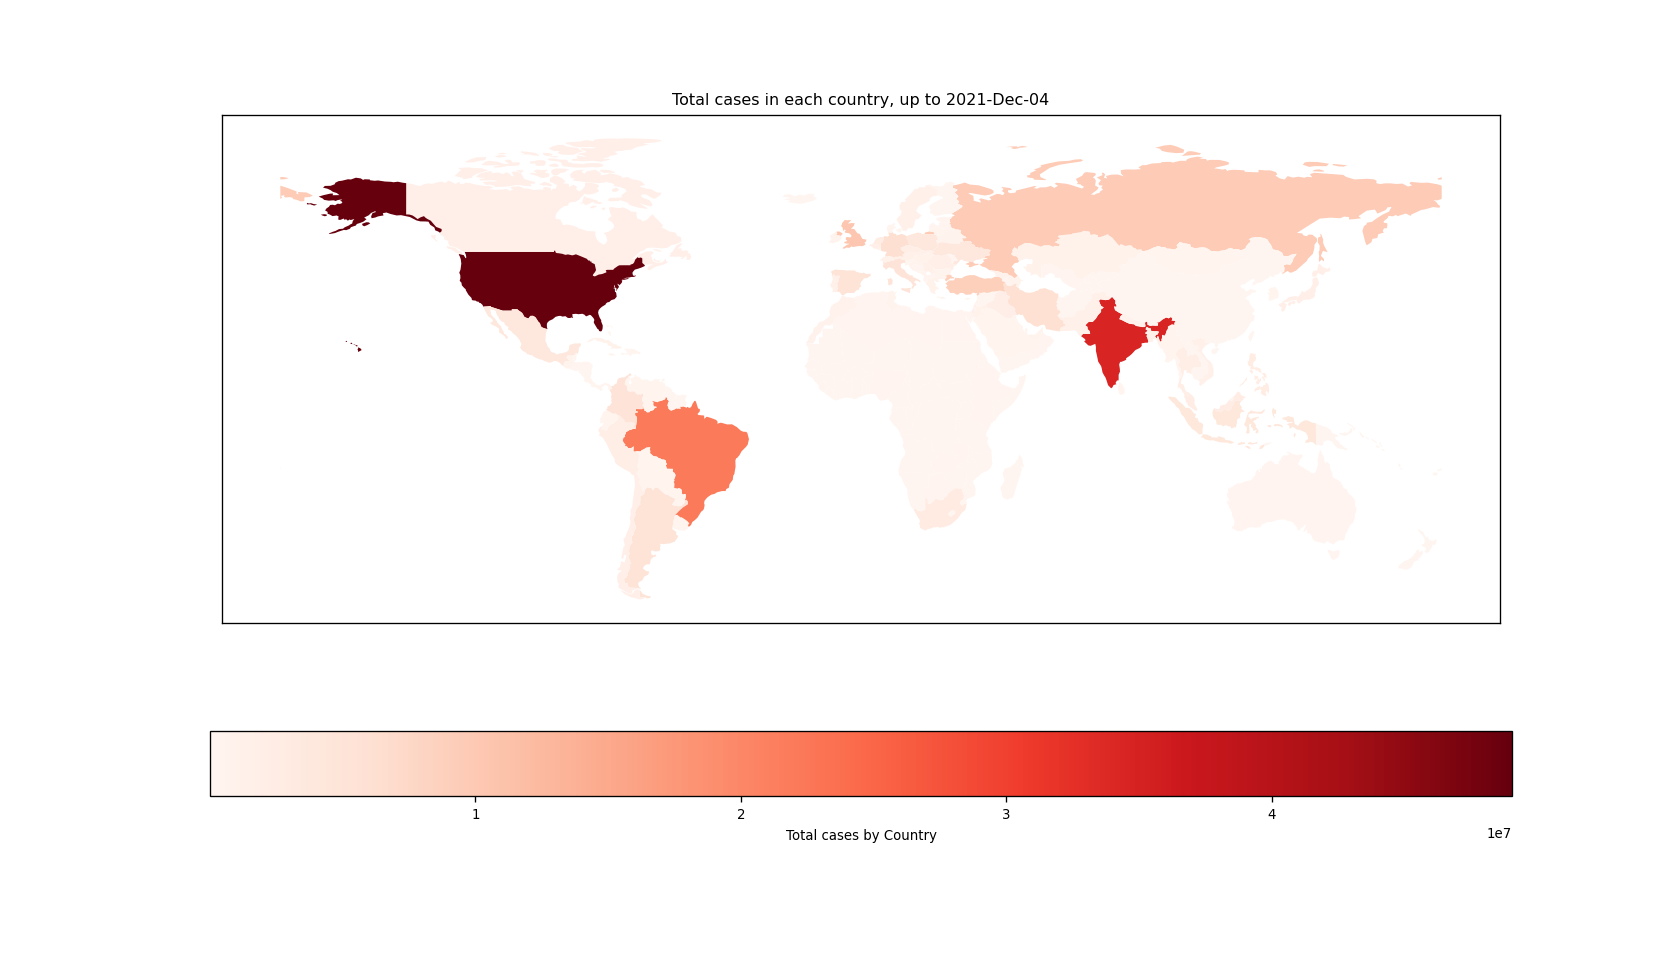
\includegraphics[width=0.9\linewidth]{../figures/total-cases-heatmap.png} % Figure image
	\caption{This figure displays the total confirmed COVID-19 cases (up to Dec 4th, 2021) of each country indicated by the darkness of the color. Countries with the most cases are the US, India, and Brazil.}
\end{figure}

\section{Exploratory Data Analysis}
This dataset has both group and timely ordered structures. Figures 1, 2, and 3 are included in this report visualizing the information extracted from a thorough EDA process. 


\begin{figure}[htb]
	\centering
	\subfigure[New Cases Original]{
		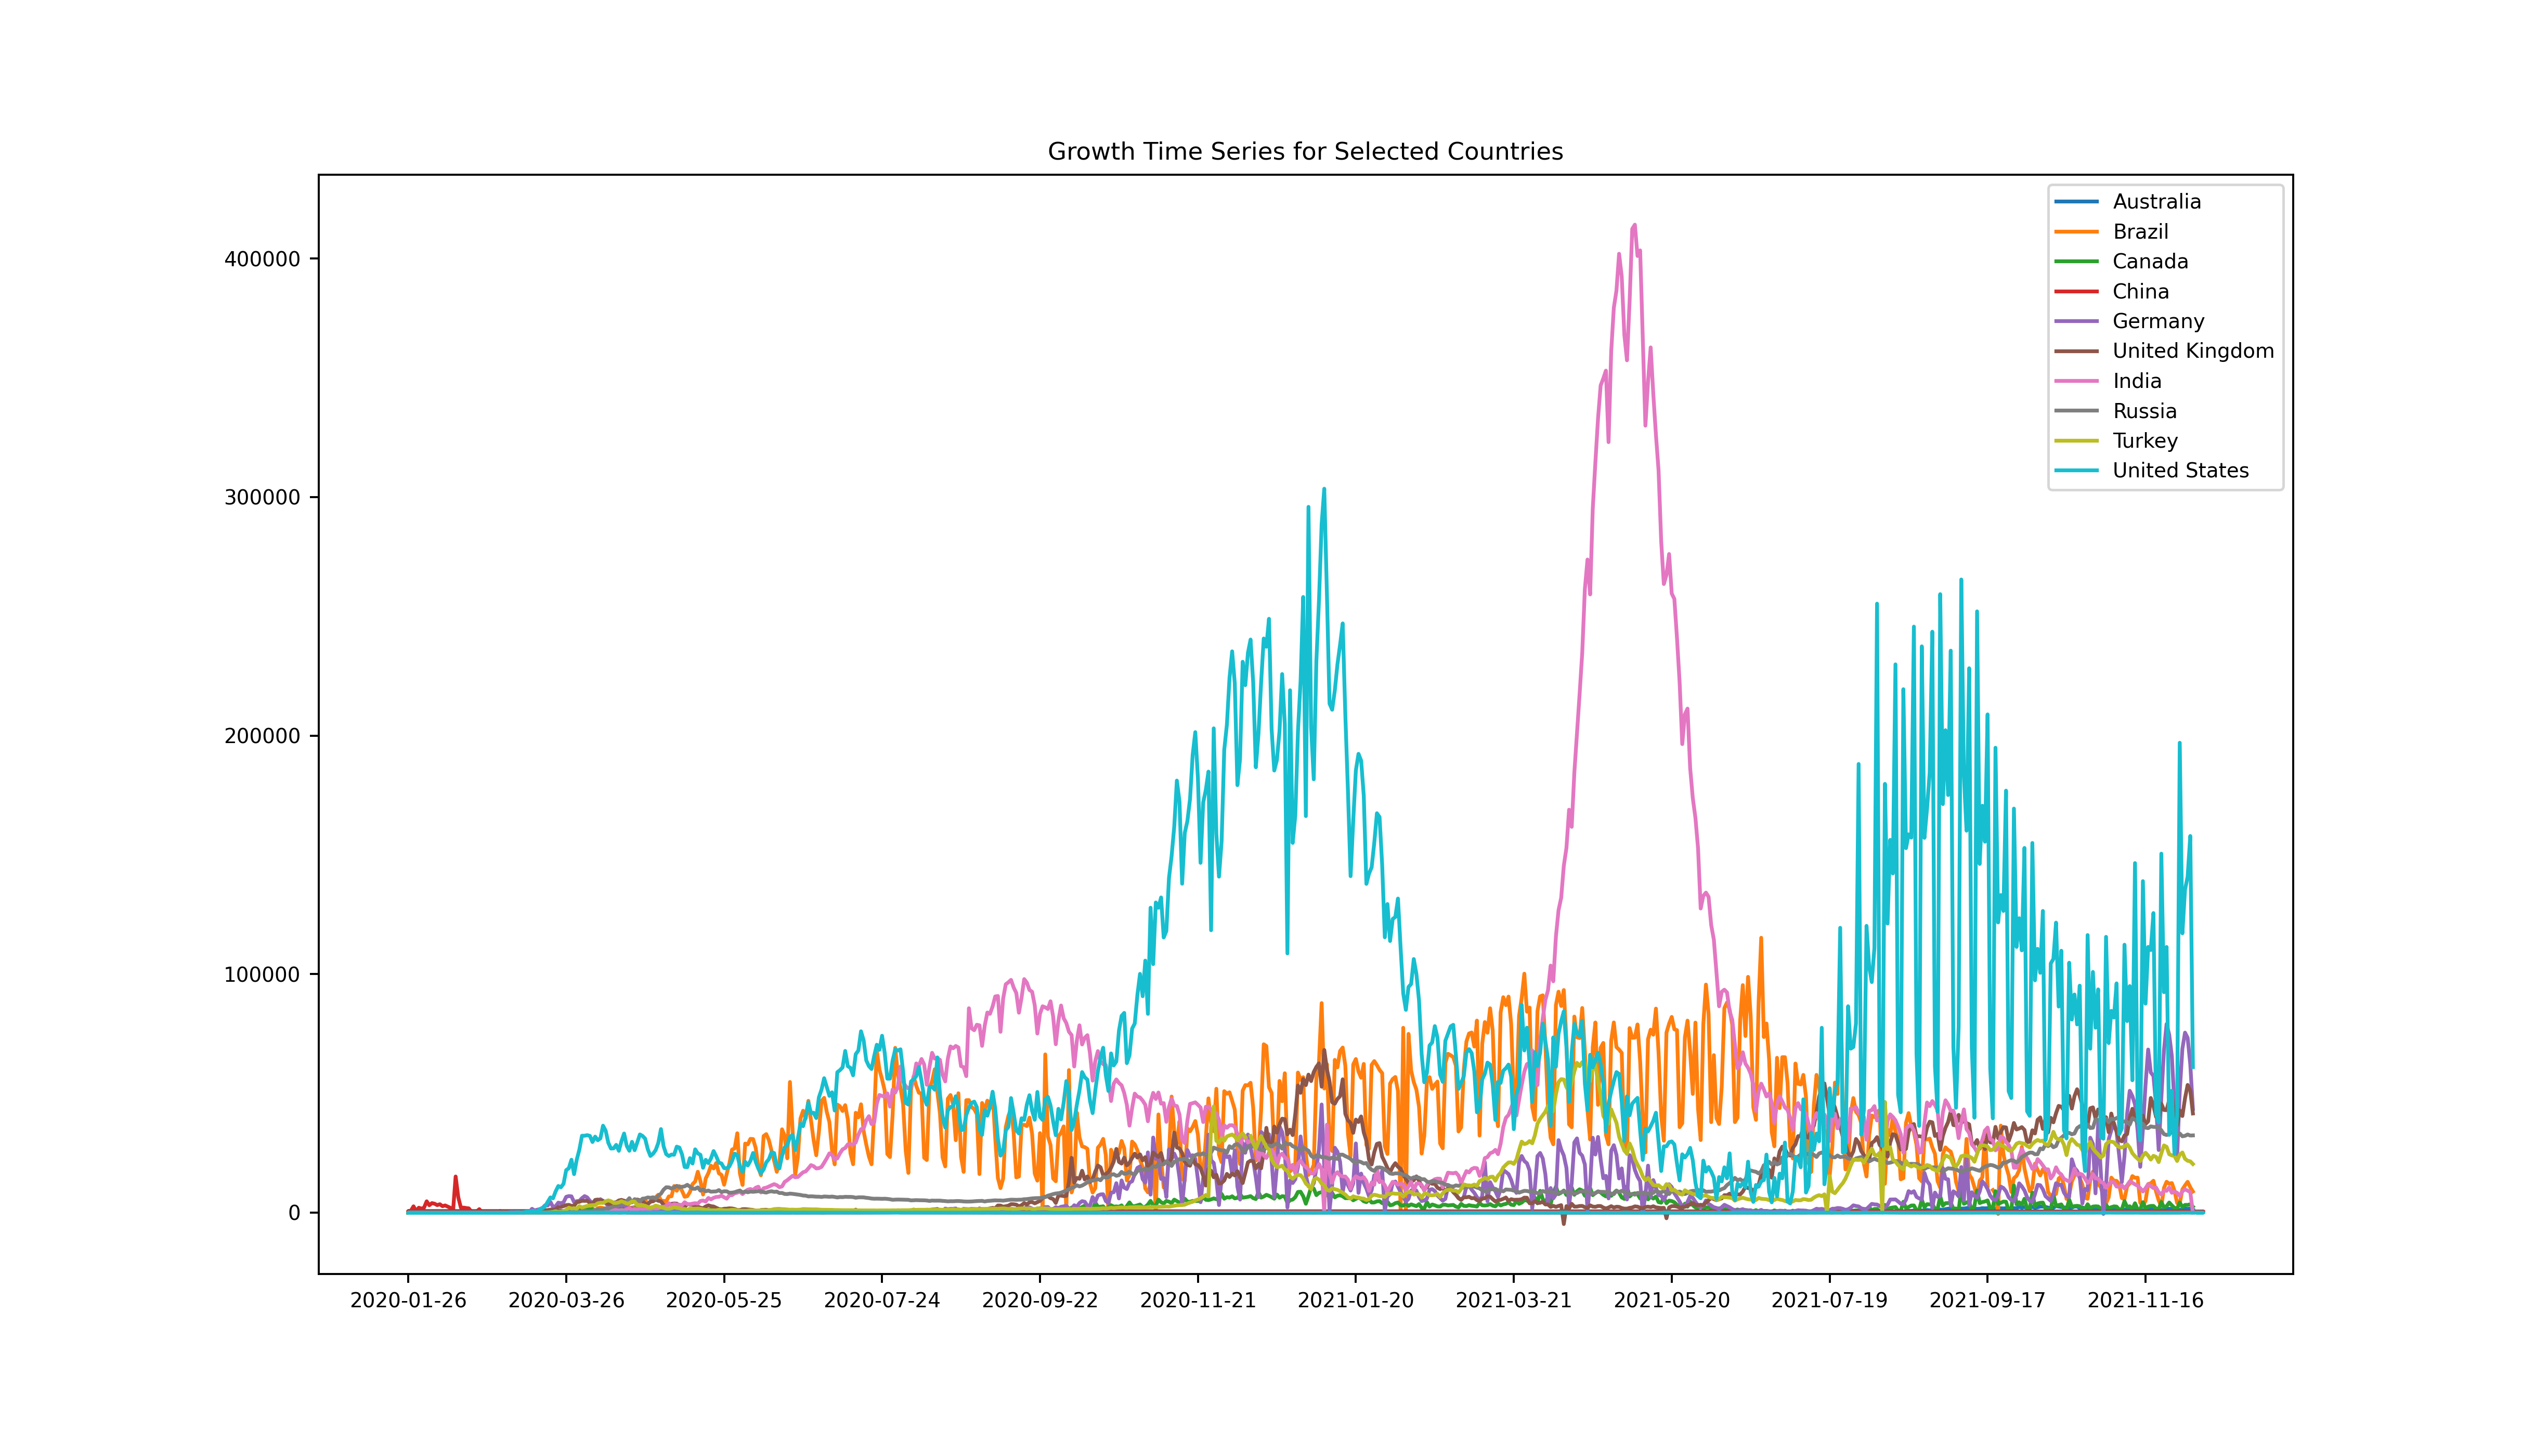
\includegraphics[width=0.5\textwidth]{../figures/new-cases.png}}\vspace{-0.1in}\hspace{-0.3in}
	\subfigure[New Cases Smoothed]{	
		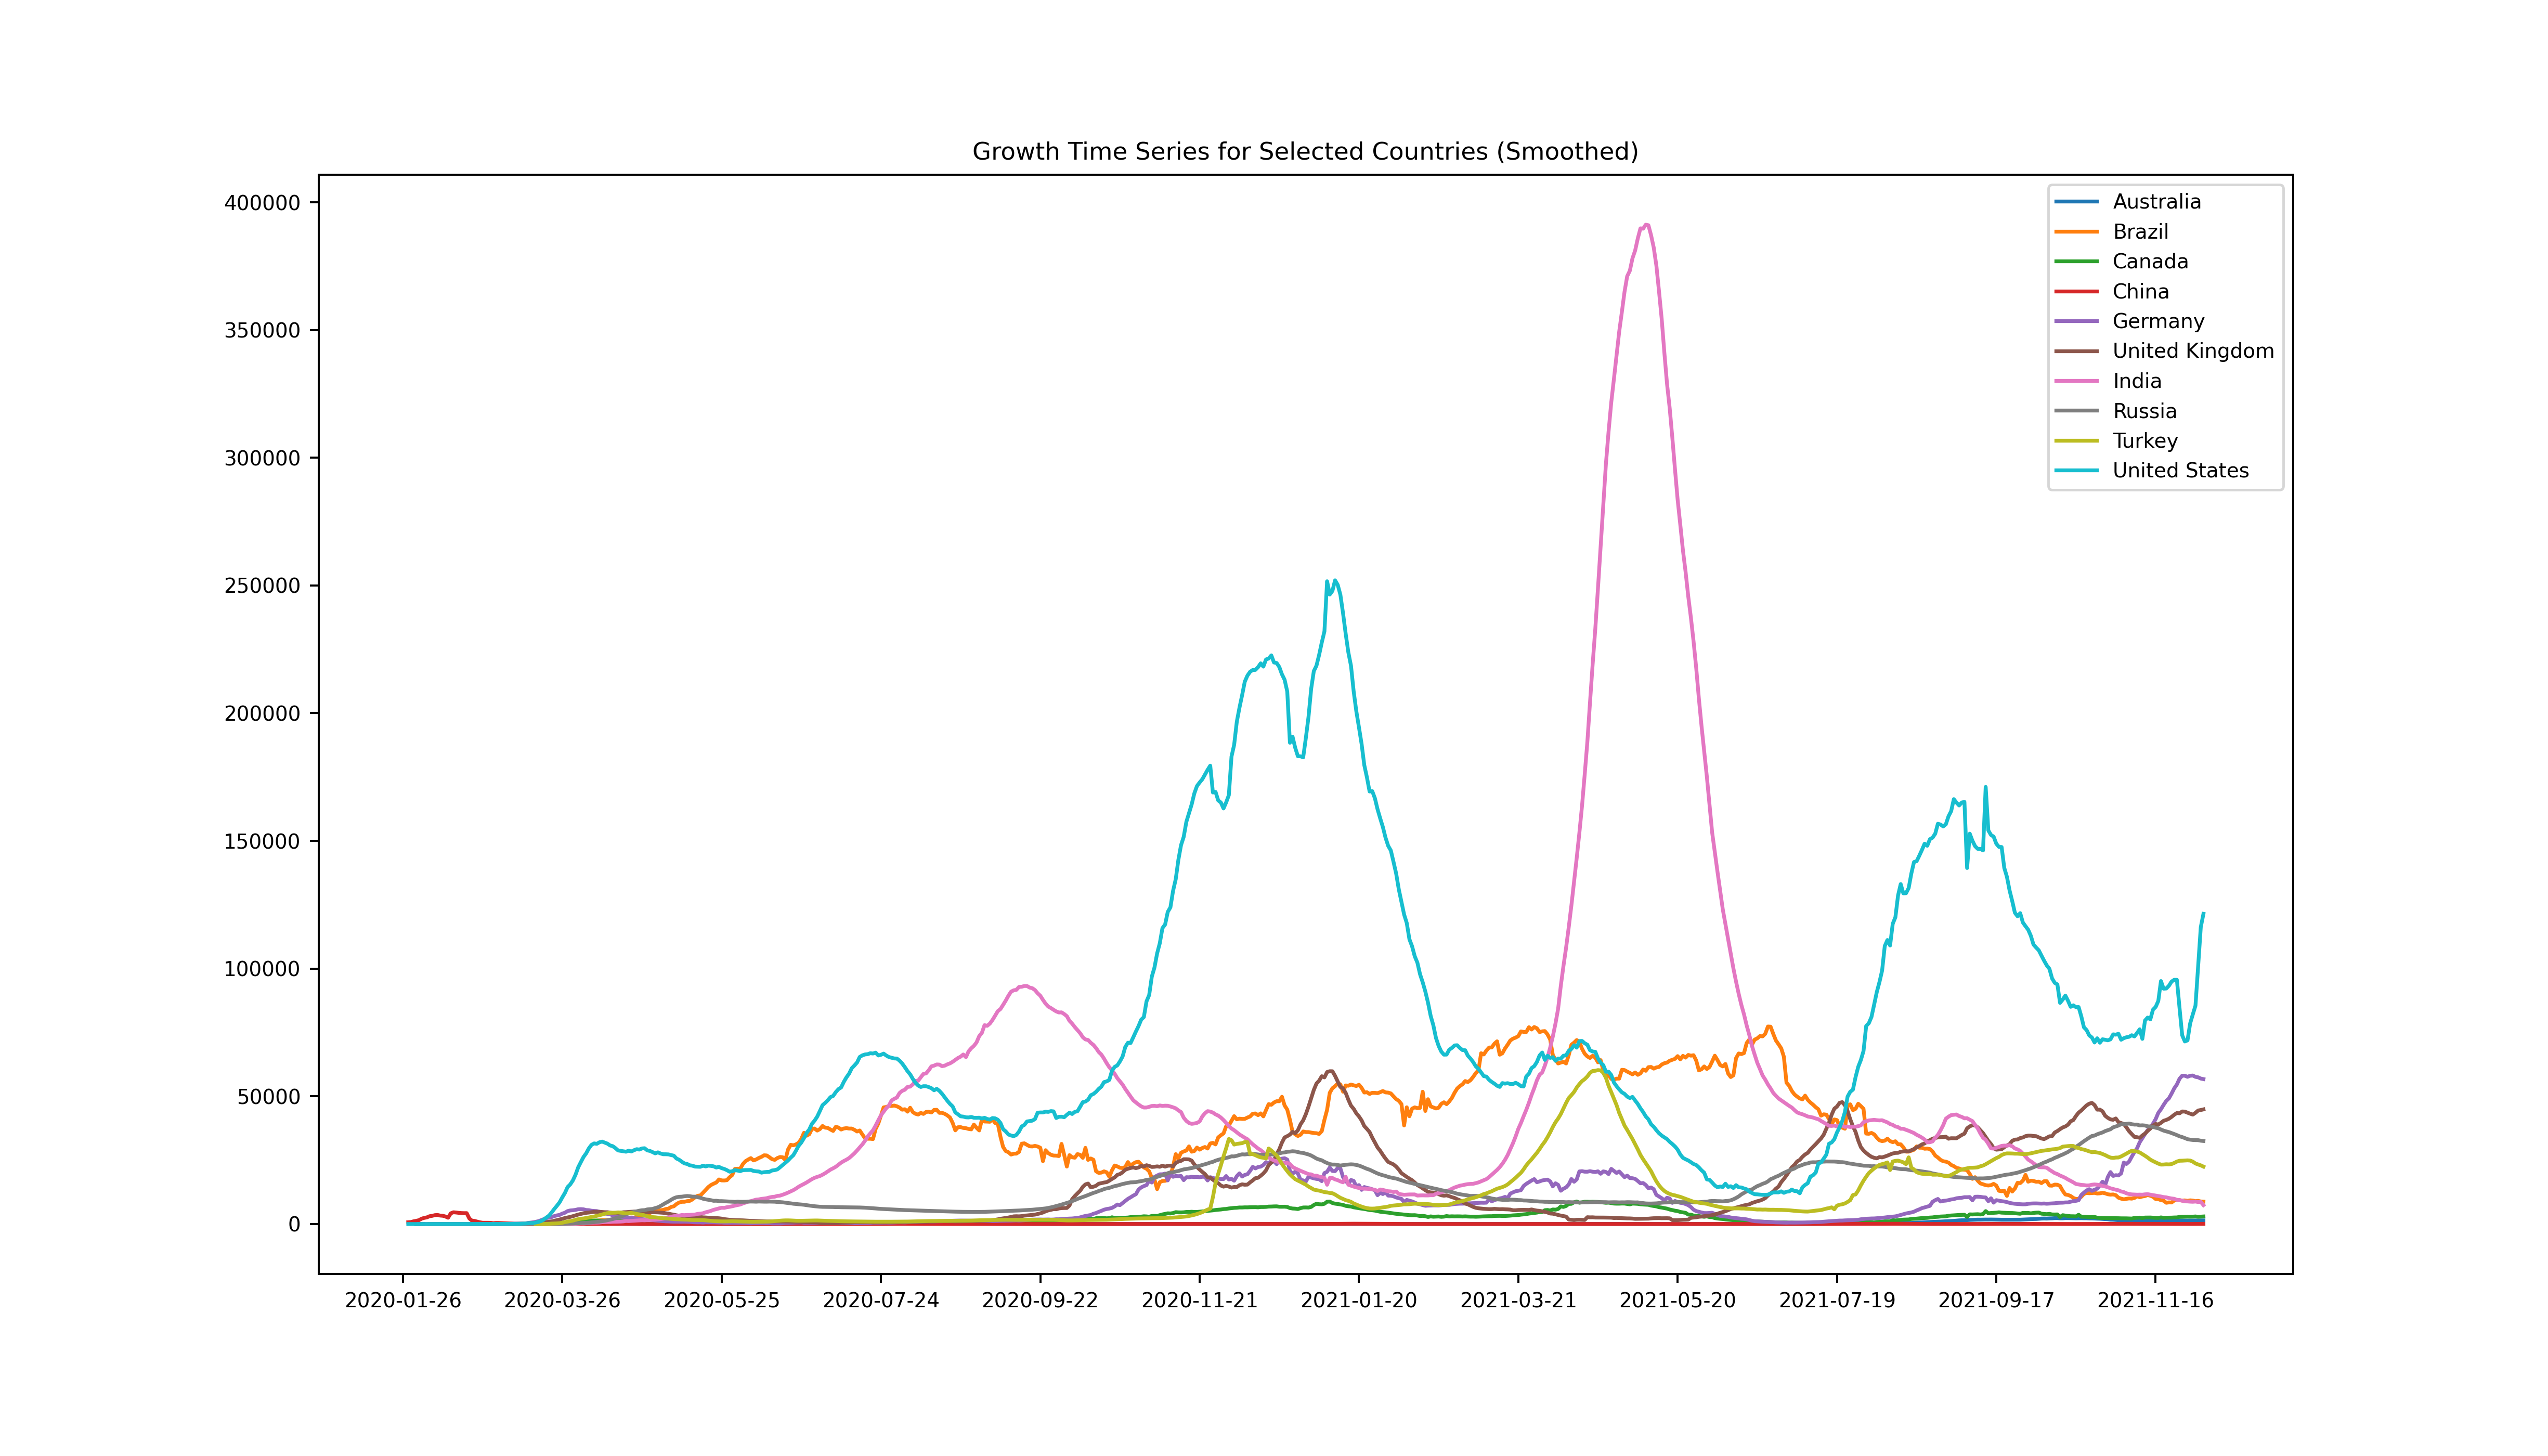
\includegraphics[width=0.5\textwidth]{../figures/new-cases-smoothed.png}}
	\caption{The two subgraphs display the growth curve of new cases from Jan 2020 to Dec 2021. The number of daily new cases is this project's target variable. We'll focus on the 7-day smoothed values (b) instead of original values (a), as there might be unexpected periodic fluctuation in the original series due to political or medical weekly reports.}
\end{figure}

\begin{figure}[htb]
	\setlength{\abovecaptionskip}{0.5cm}
	\centering
	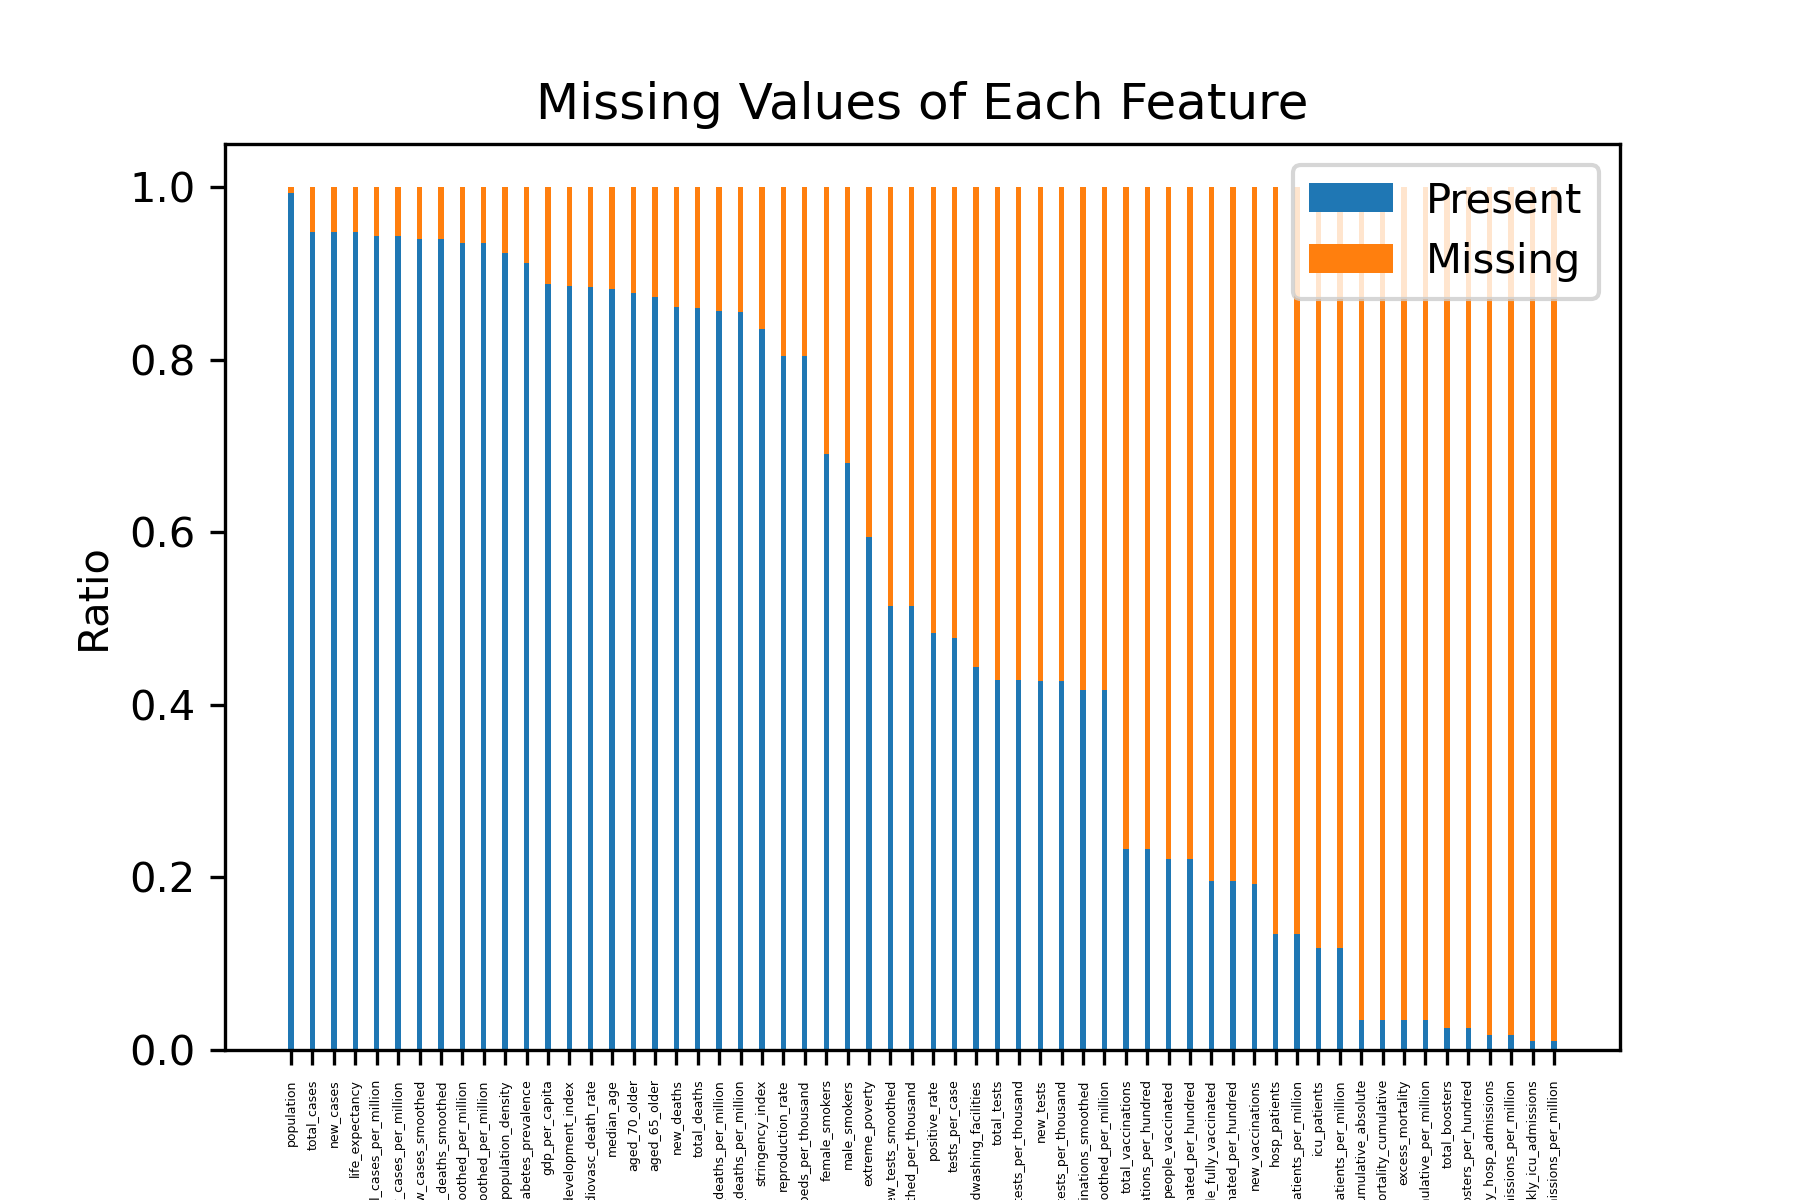
\includegraphics[width=0.6\linewidth]{../figures/missingvalues.png} % Figure image
	\caption{All columns have missing values. Over 90 percent of data in the right most ten features are missing. Those columns are dropped in the following machine learning models.}
\end{figure}



\section{Methods}
The task is to forecast future new cases (smoothed within a 7-day window) and provide a universal analysis pipeline for predicting new cases in different countries. The following part will focus on data from the United States as an example. The training and validation set of USA data contains 628 records previous to 2021-10-10 (submission date of the midterm proposal), and the testing part includes the most recent 55 records from 2021-10-11 to 2021-12-04.

\subsection{Supervised models}

By grouping on countries, we get different time-series data. In feature selection, columns directly related to the target variable (those concerning new cases data) are eliminated, leaving 53 features eligible for the training process. Further more, three properties regarding missing values can be drawn from the OWID dataset, and give us a handle to deal with missing values.
\begin{enumerate}
	\item If the missing values are present at earlier dates, it might be due to not detected cases, which can be replaced with zeros.
	\item Many columns have a large proportion of missing values, and over 95 percent is missing in features like weekly hospital admissions and excess mortality. So those columns are not actually informative and can be dropped.
	\item Some columns are manipulated from an original one for comprehensive use, e.g., the new deaths cases are smoothed, integrated, or divided by the population to generate smoothed trends, total cases, and death rates. Thus, only keeping the originally collected data is enough for the machine learning models.
\end{enumerate}
After preprocessing, 23 features are kept in total. In terms of splitting and cross validation, we should never fit future data to predict previous points in time series, so the training set should only contain records previous to those in the test set and the same for the validation set. My cross validation splitting strategy is shown in Figure 4. Then standard scaler is applied on the 23 selected features inside the loop of K-Fold, where $K$ is set as 4. The best combination of hyperparameters is tuned on validation RMSE scores.\\

The baseline model is Linear Regression. Additional regression models include SVR and XGBoost. Note that time series fed into the XGBoost model are not imputed for missing values.
\begin{figure}[htb]
	\setlength{\abovecaptionskip}{0cm}
	\centering
	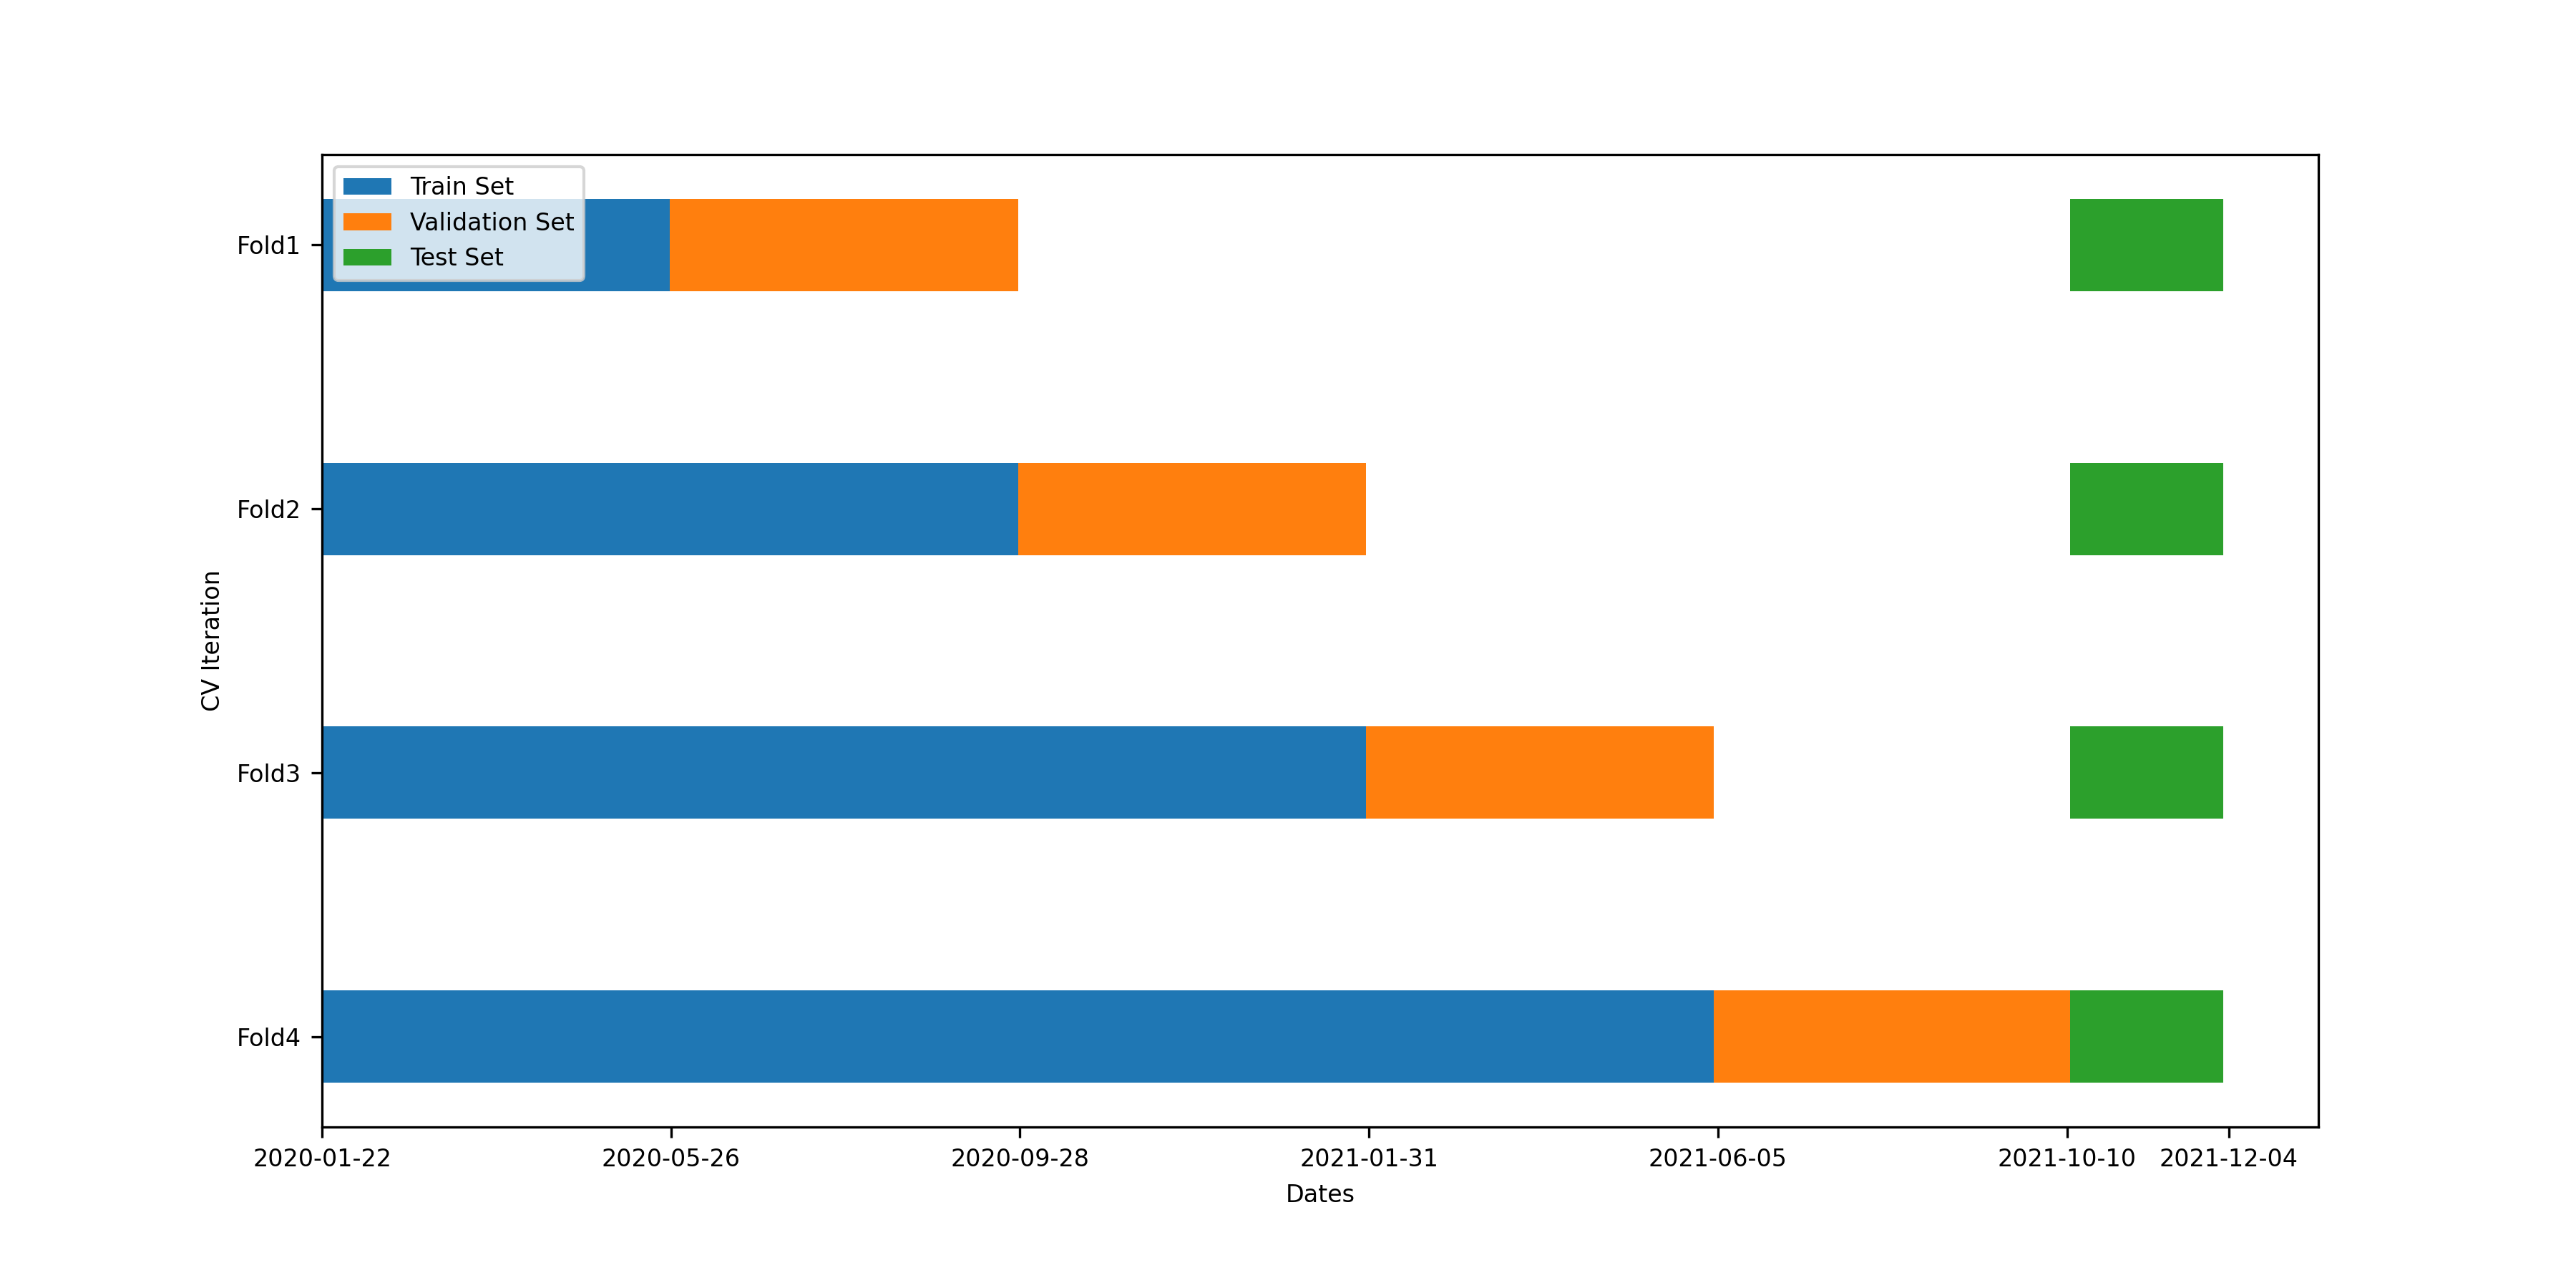
\includegraphics[width=0.8\linewidth]{../figures/Cross-validation.png} % Figure image
	\caption{Splitting the training time series for 4-Fold cross validation} 
\end{figure}



\subsection{Time Series Analysis}
ARIMA$(p,d,q)$ models can be applied on time series to predict future trends with a linear combination of past data (Auto-Regression part) and independent white noises (Moving Average part). As ARIMA requires the series to be stationary, differencing the original series is one strategy to meet that need. To decide a grid searching scale of the three hyperparameter -  the orders of difference, auto-regression, and moving average - a general method is to detect a cut-off time lag from the PACF (Figure 5) and ACF (Figure 6) graphs on the training series.\\

ARIMA is different from other supervised machine learning models as it only takes one variable as input, trying to find a trend or pattern from the target series itself. Similar to supervised models, ignoring the starting NAN values won't have much influence on the result. \\
 
Tuning hyperparameters $p,q$ of ARIMA is based on the AIC values, know as Akaike information criterion. The reason for not using RMSE as the validation metric is that AIC takes both the log-likelihood and model complexity into account by giving a penalty on the order of AR and MA parts. 
 \begin{figure}[htb]
 	\setlength{\abovecaptionskip}{0.cm}
 	\centering
 	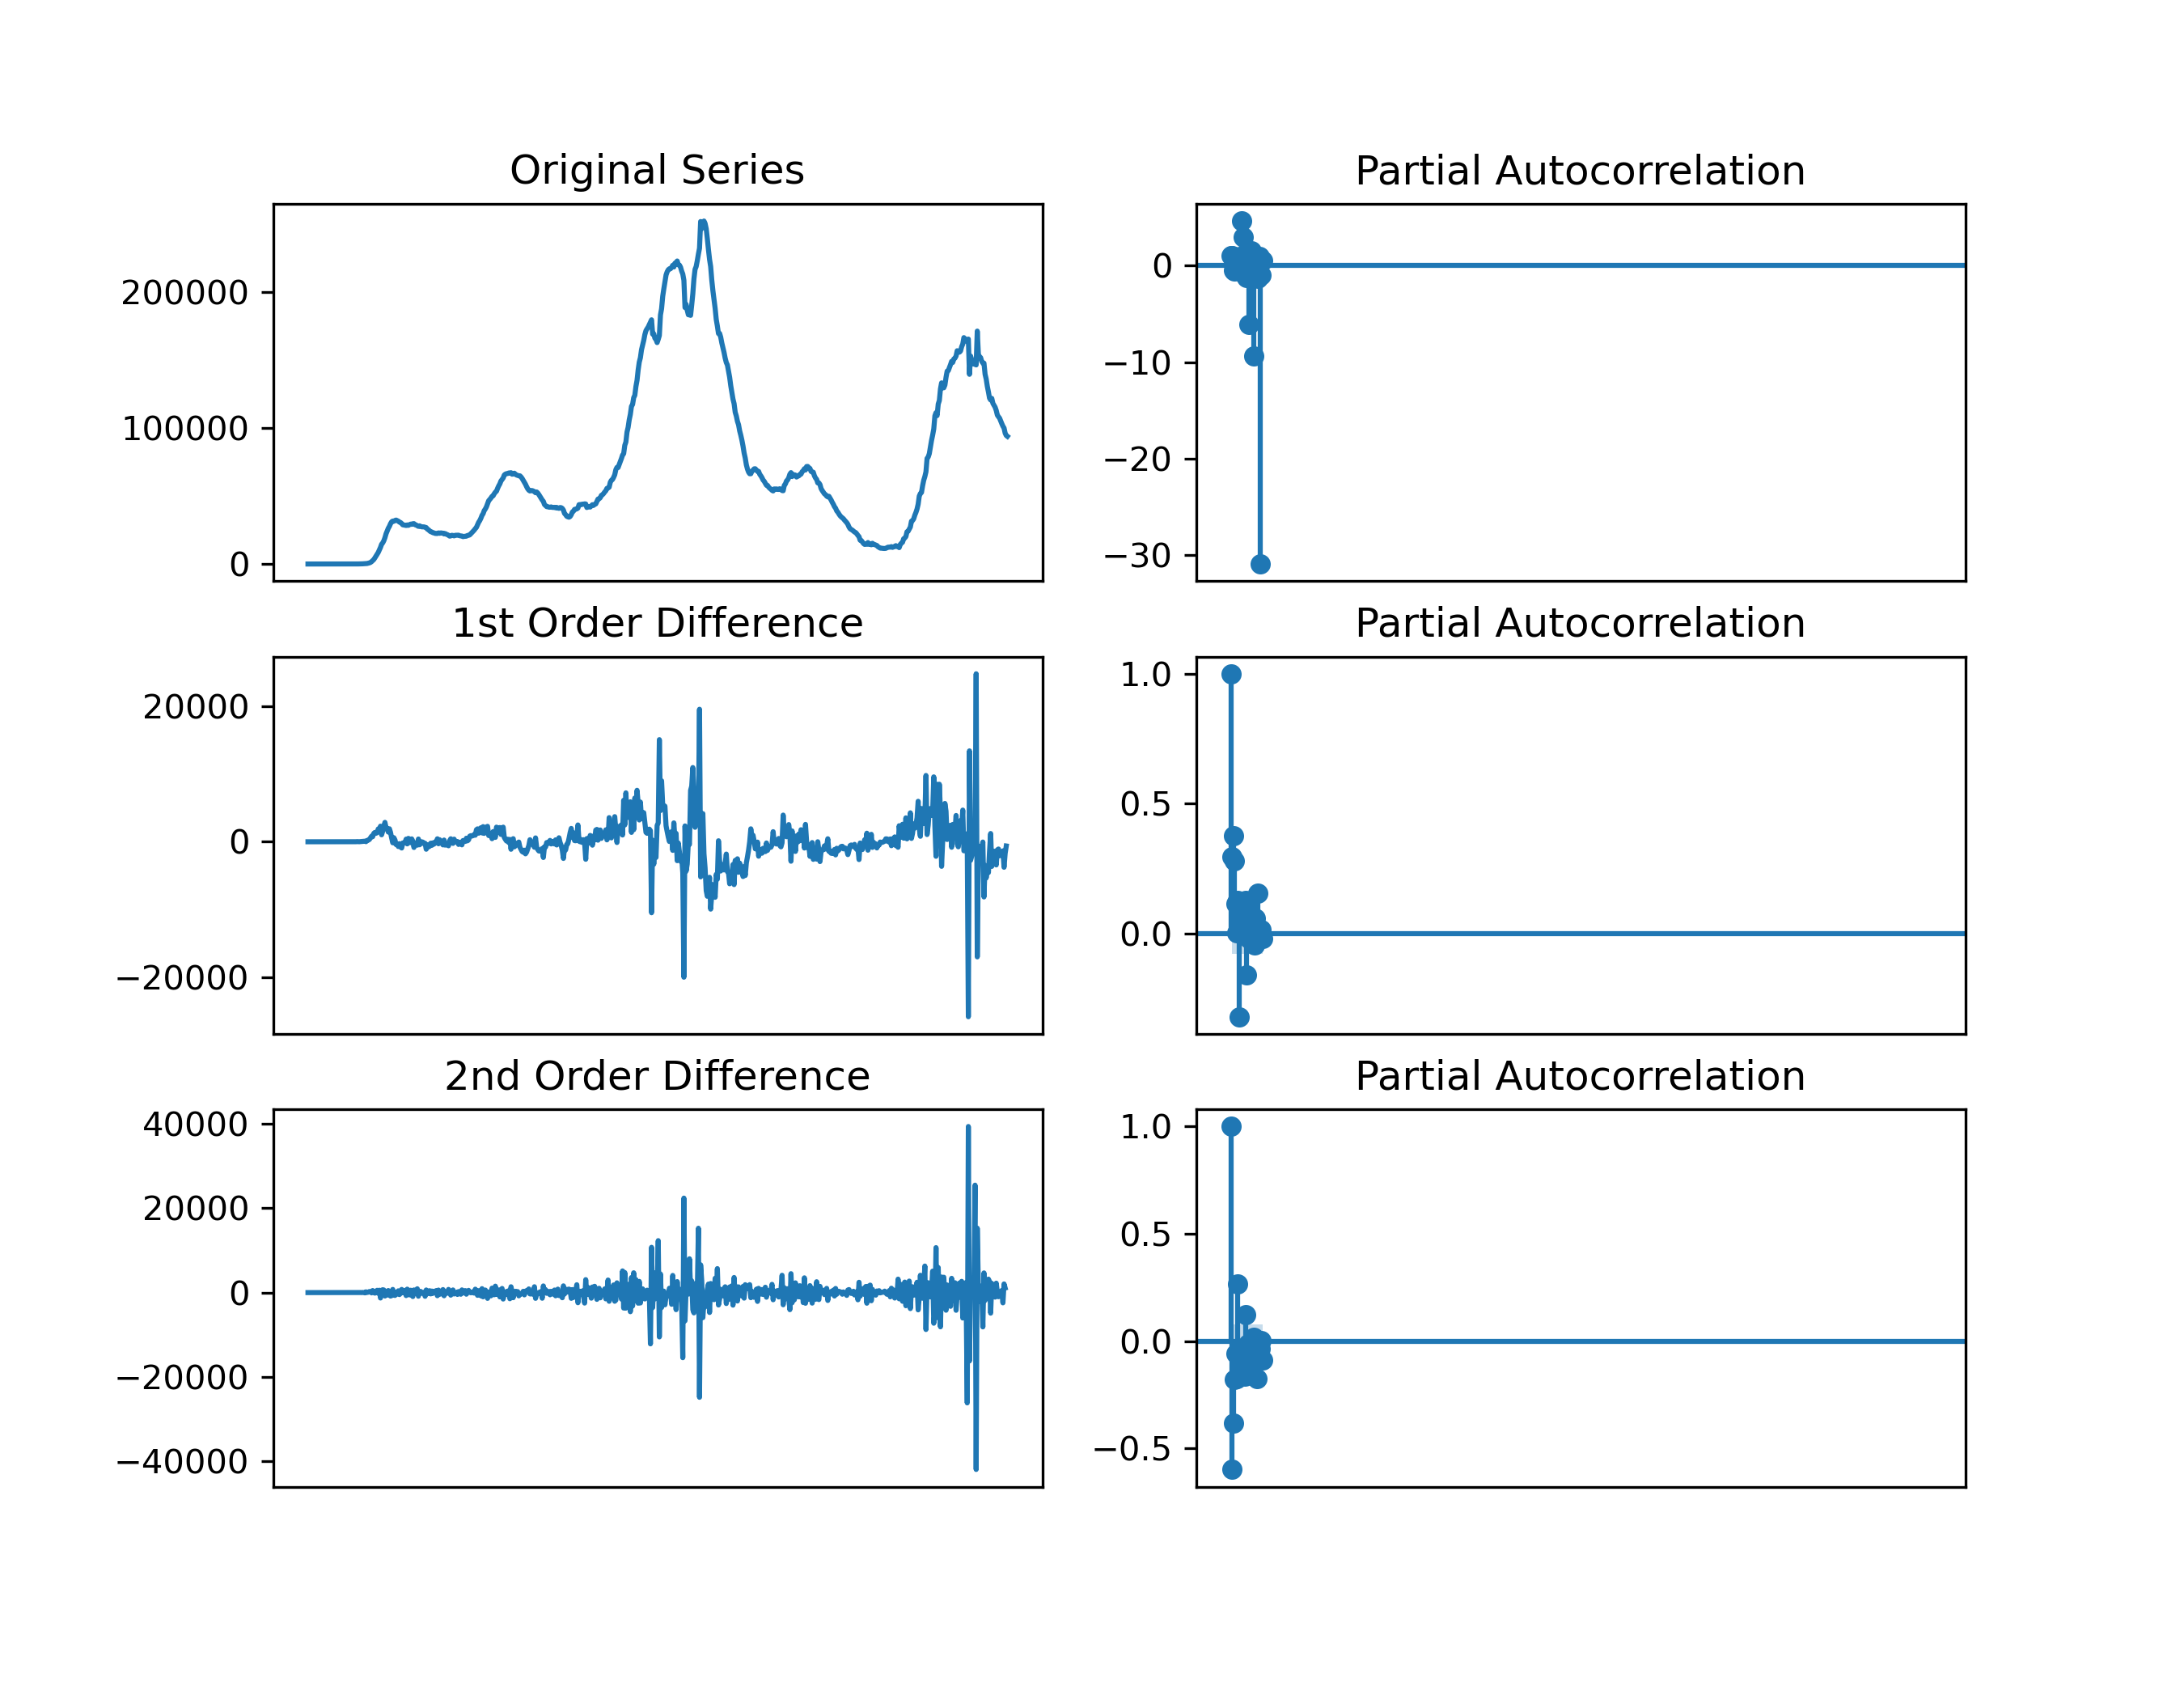
\includegraphics[width=0.8\linewidth]{../figures/PACF.png} \vspace{-0.3in}
 	\caption{By differencing the original series several times, the generated series will gradually become stationary. While the 2nd order difference series is the most stationary among the three, there is a probability that it might be over-differenced. So 1st order difference is fed to the ARIMA model ($d=1$). PACF graphs in the right part indicate the choice for order of auto-regression term $p$ according to the cut-off lag. The maximum value of $p$ is set as 5.}
 \end{figure}
 
 
 
 \begin{figure}[htb]
 	\setlength{\abovecaptionskip}{0.cm}
 	\centering
 	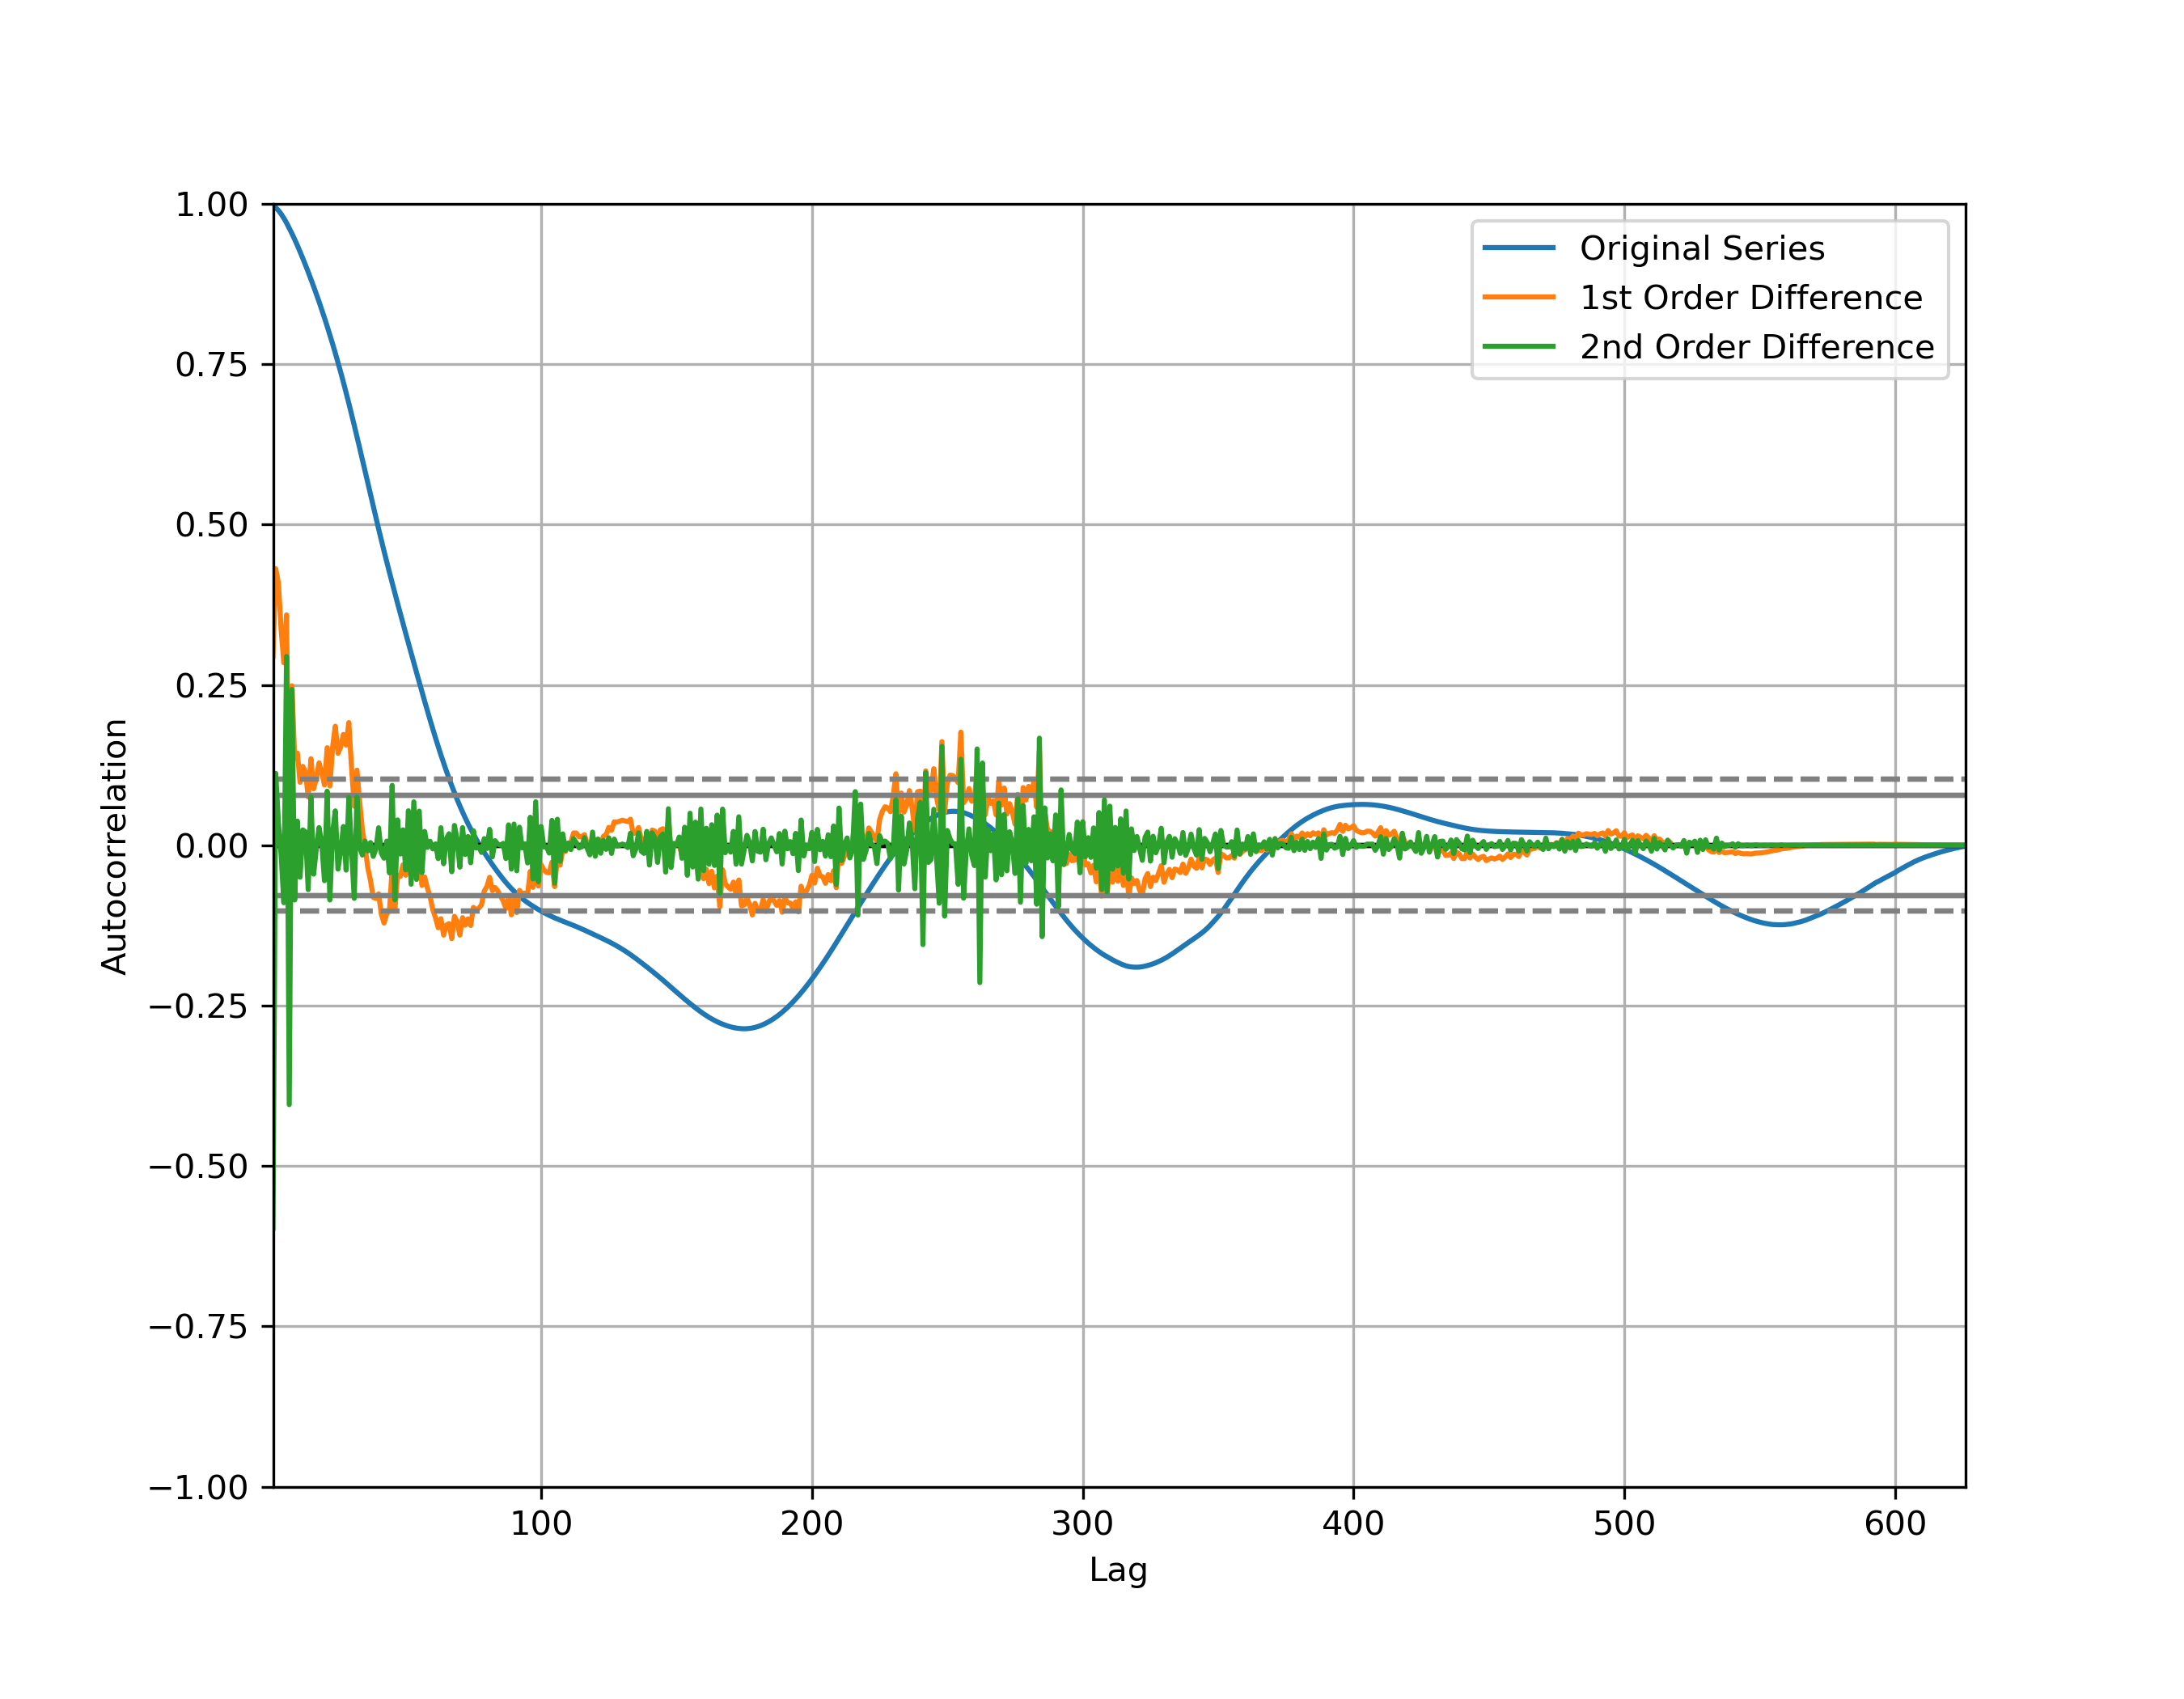
\includegraphics[width=0.6\linewidth]{../figures/ACF.png} \vspace{-0.1in}
 	\caption{The ACF graph indicates the order of moving average term $q$. In the orange curve, while several points after lag 10 are still statistically significant, lying outside the gray threshold, maximum of $q$ is set as 4 following the principle of K.I.S.S. } 
 \end{figure}


\section{Results}
\begin{table}[htbp]
	\caption{Performance of Different Models}
	\centering
	\begin{tabular}{lccc}
		\toprule
		Model & RMSE& Validation Mean & Validation STD \\
		\midrule
		Linear Regression&28912.46&	28021.60&	11681.58
		\\
		SVR&	22351.24&	63143.47&43978.68
		\\
		XGBoost&19740.74&	43910.82&	44963.51
		\\
		ARIMA&	 11977.69&-&-
		\\
		ARIMA (Rolling)&	4220.17&-&-
		\\
		\bottomrule
	\end{tabular}
\end{table}
\subsection{Supervised models}
Figure 7 illustrates the forecast results of linear regression, SVR, and XGBoost model. XGBoost best fits the training data and achieves the smallest prediction RMSE on the test set among the three models. XGBoost also successfully predicts the growing trend at the beginning of December, whose curve is also smoother, while the other two regression models show more vibration and non-stability. The four most important features of XGBoost model are reproduction rate, tests per case, new deaths, and hospital patients. The local importance is described as shap values, shown in Figure 8. A surprising fact is that the feature of tests per case is negatively influencing the new cases.\\

However, one might be concerned about the plausibility of supervised models. When forecasting future trends (the target), those models take corresponding features of future data as input, which are also inaccessible from the current view. So time series models might be more suitable to apply for this task.
\begin{figure}[!htb]
	\centering
	\subfigure{
		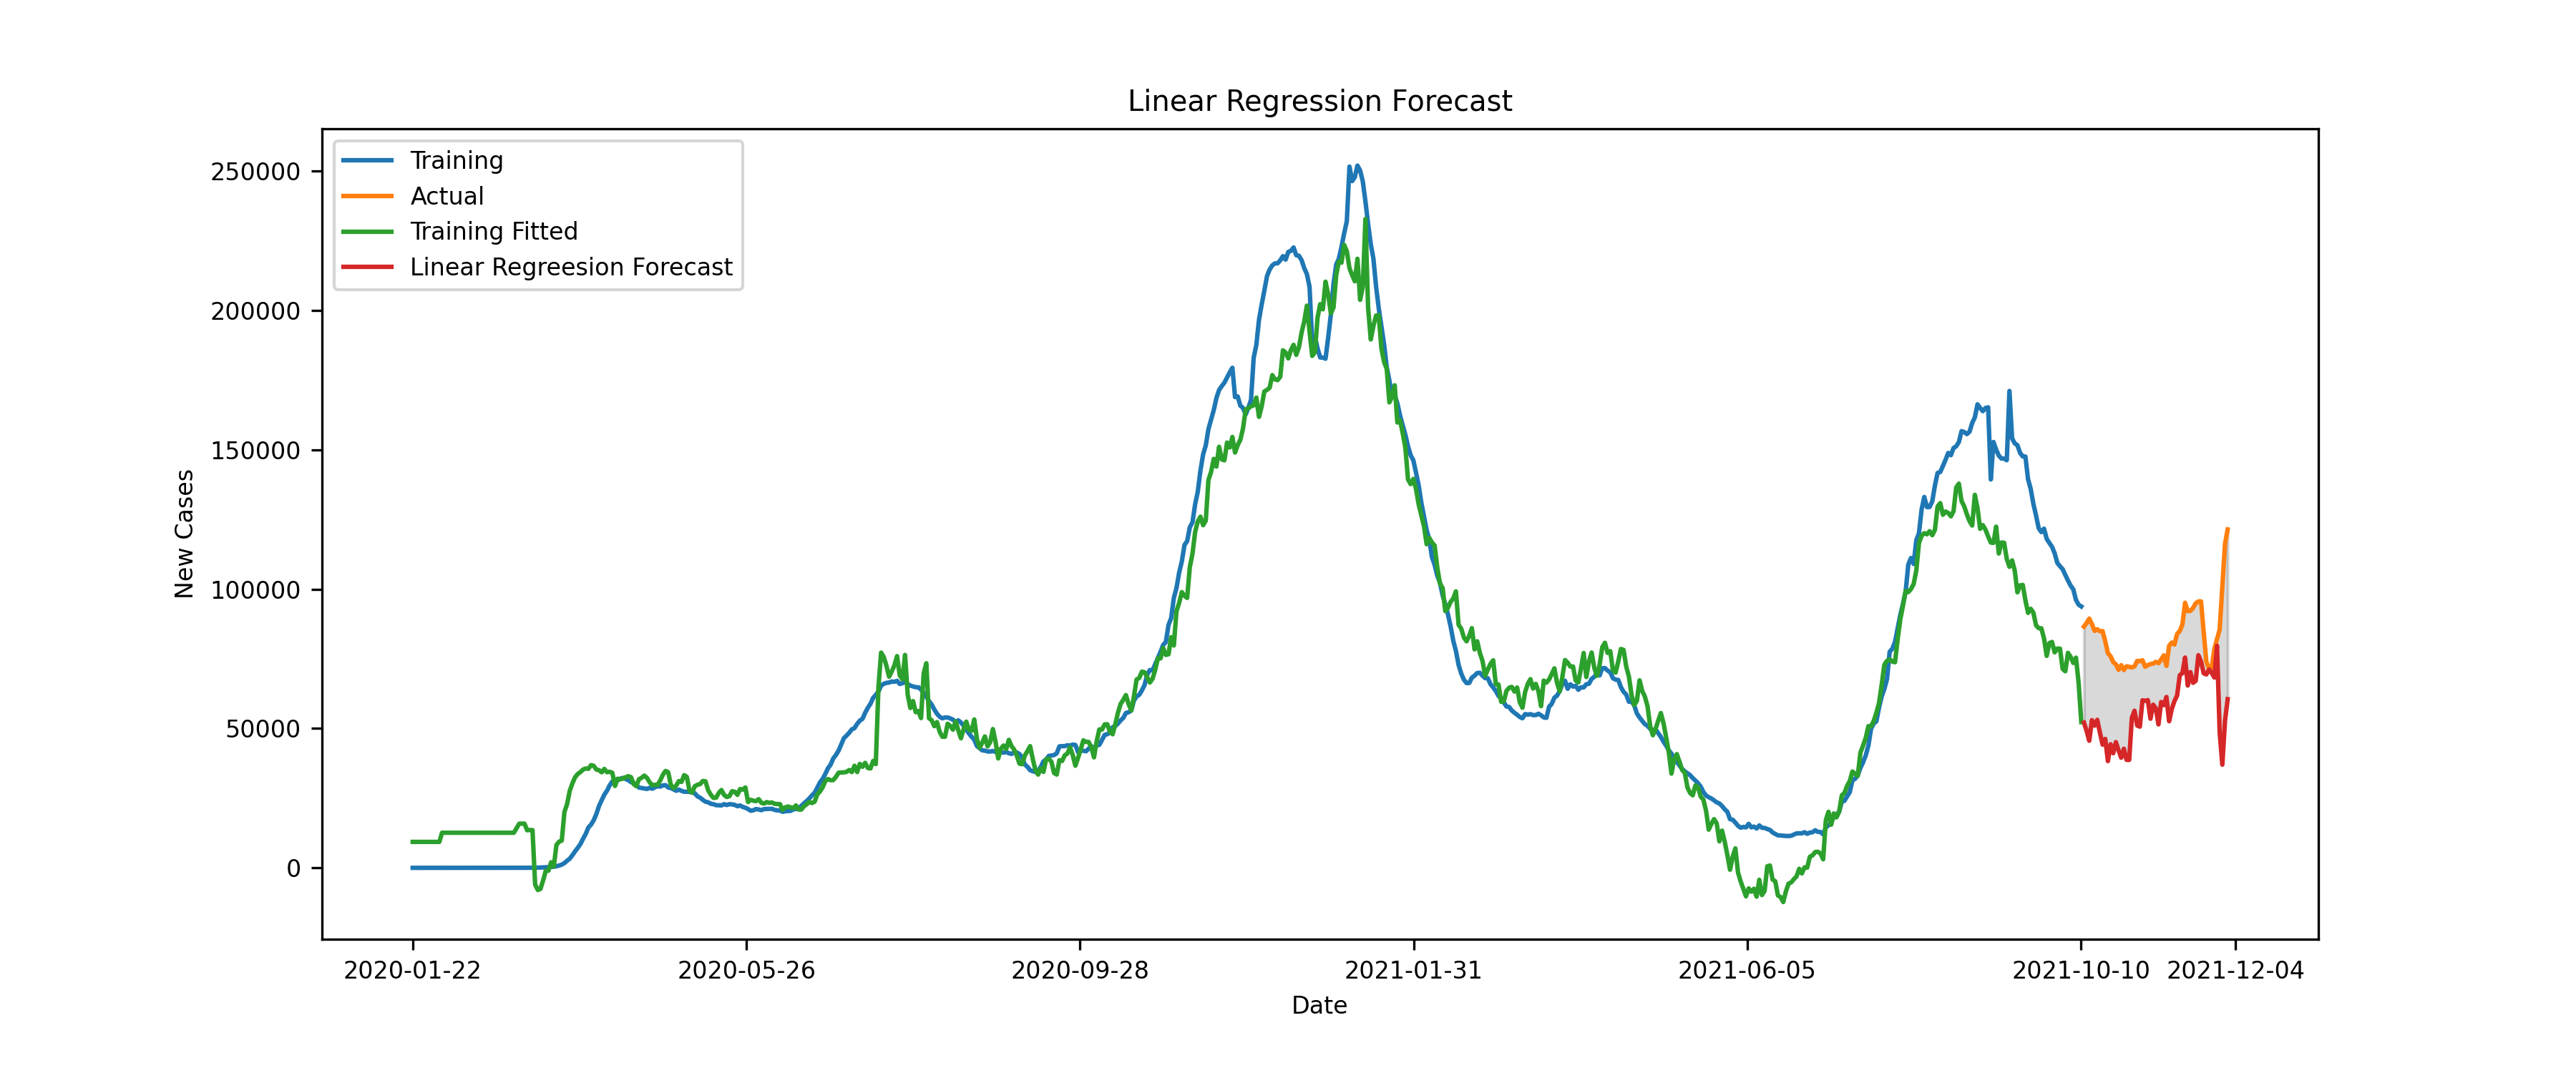
\includegraphics[width=0.9\textwidth]{../figures/LinearModel.png}}\vspace{-0.3in}
	\subfigure{	
		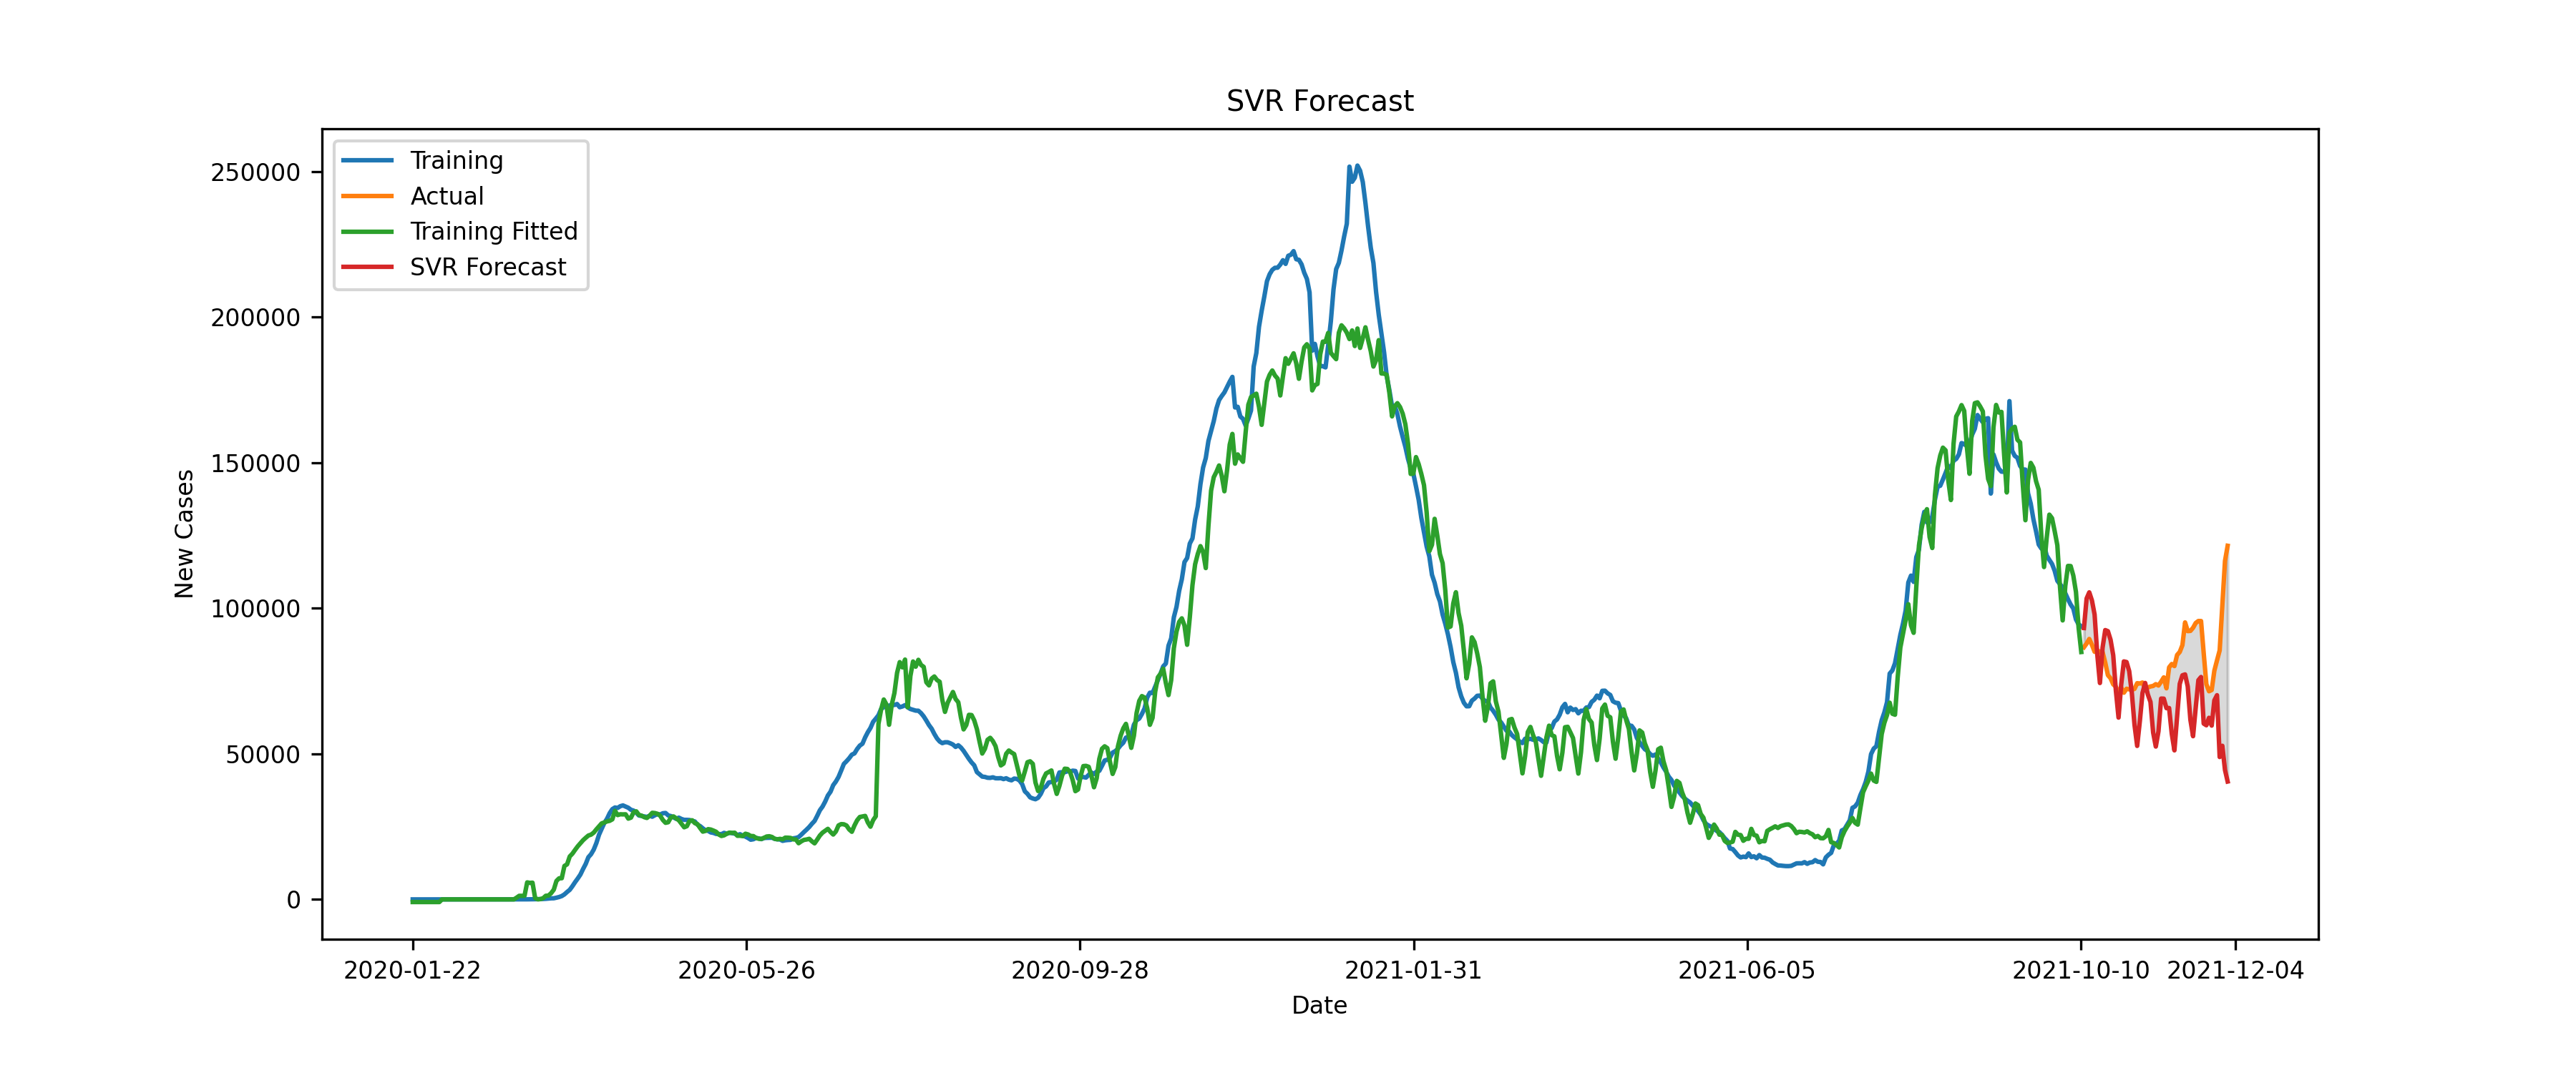
\includegraphics[width=0.9\textwidth]{../figures/SVRModel.png}}\vspace{-0.3in}
	\subfigure{	
		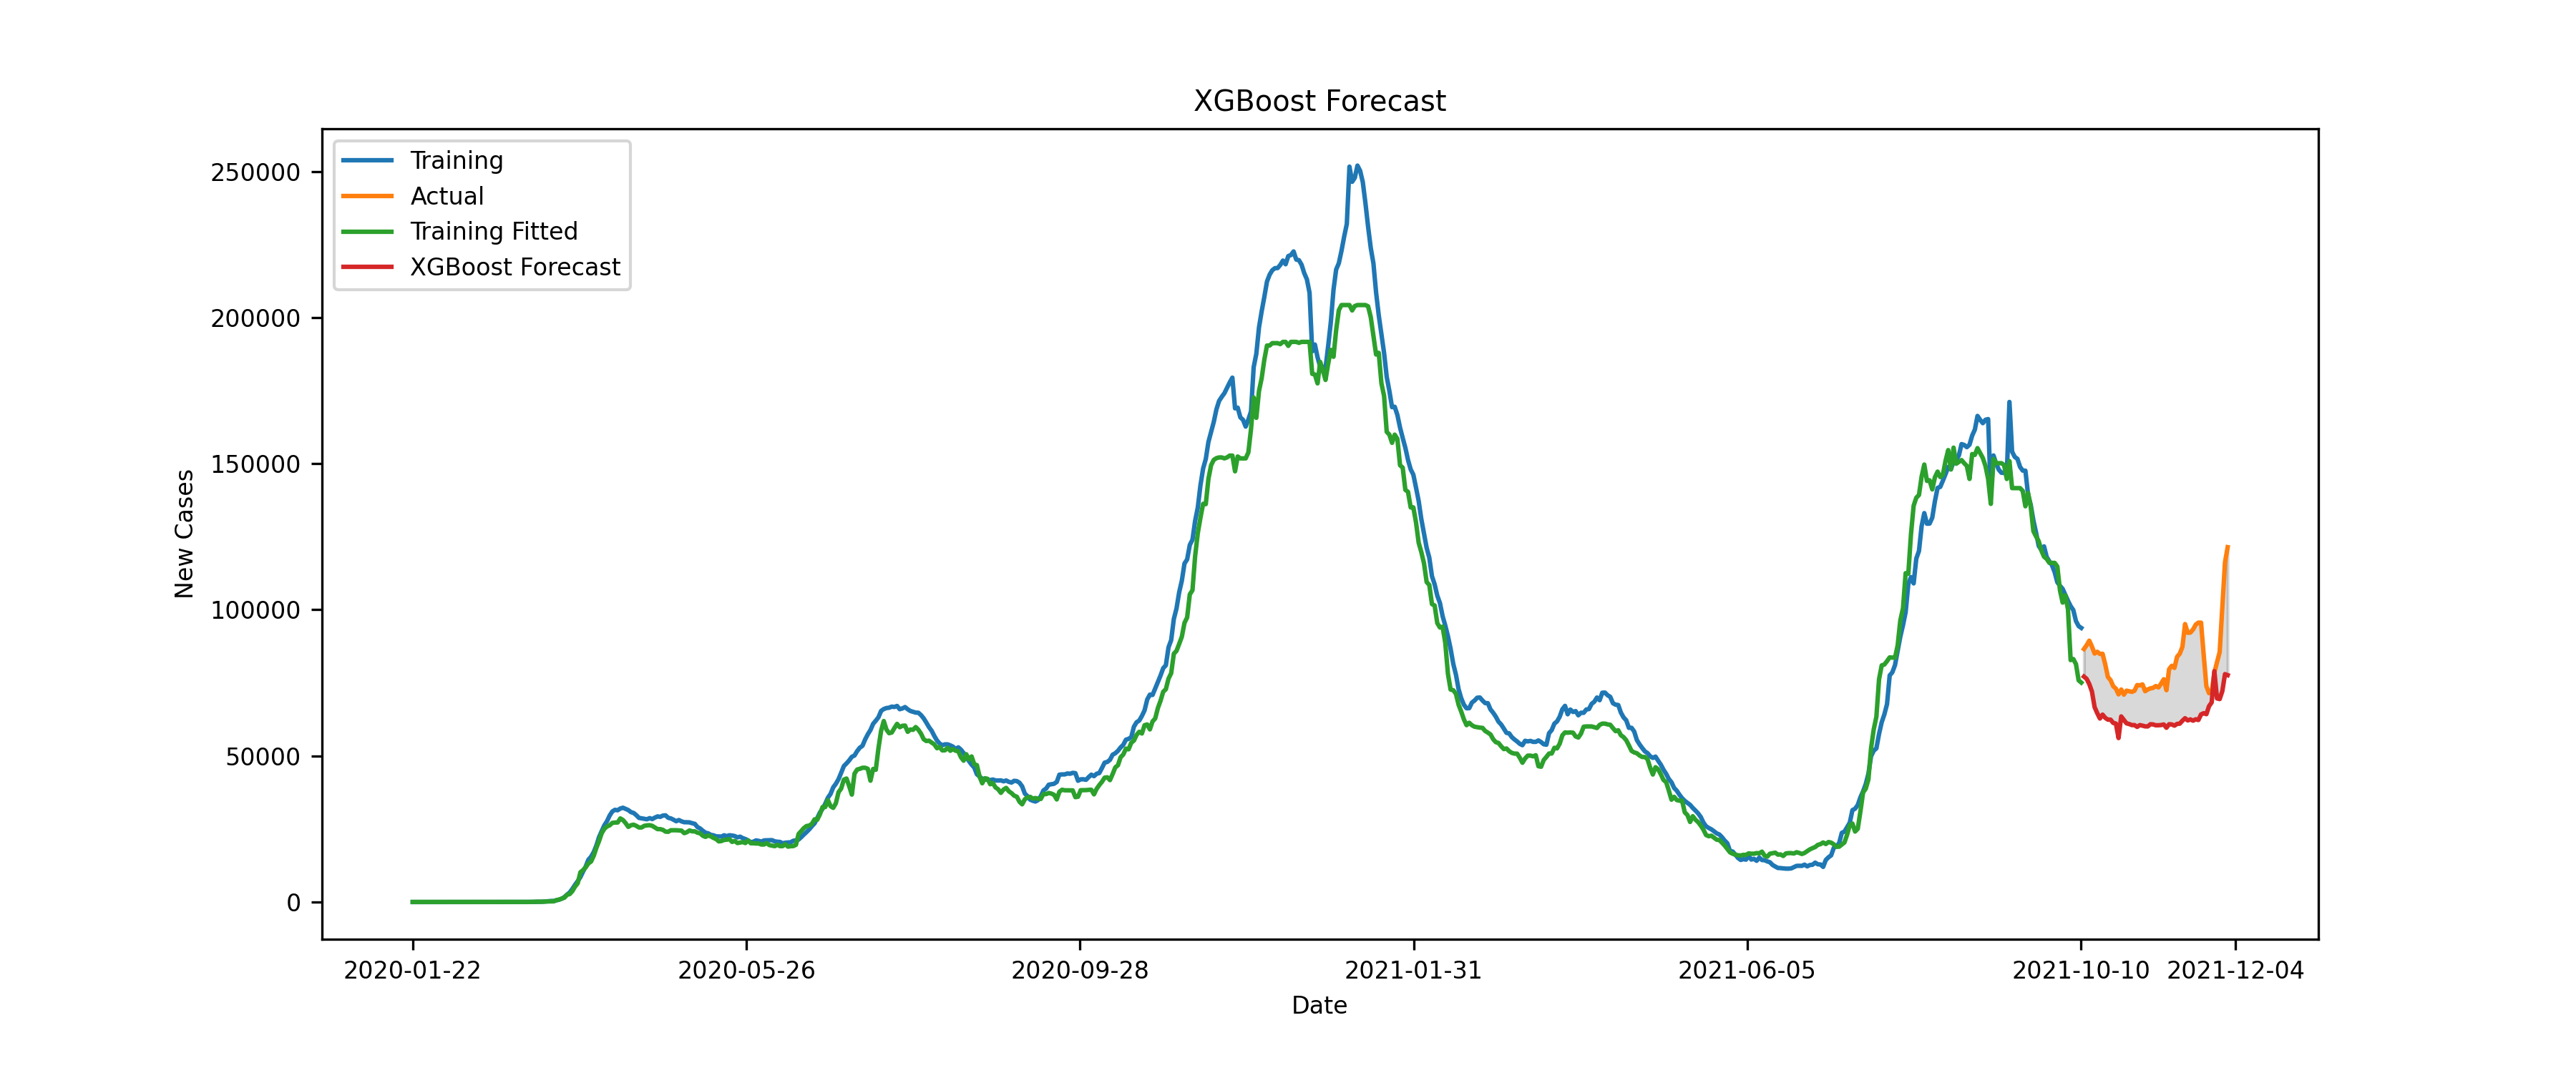
\includegraphics[width=0.9\textwidth]{../figures/XGBoostModel.png}}\vspace{-0.1in}
	\caption{XGBoost model beats linear regression and SVR, showing the best performance both in trend fitting and smoothness.}
\end{figure}

 \begin{figure}[!htb]
	\setlength{\abovecaptionskip}{0.cm}
	\centering
	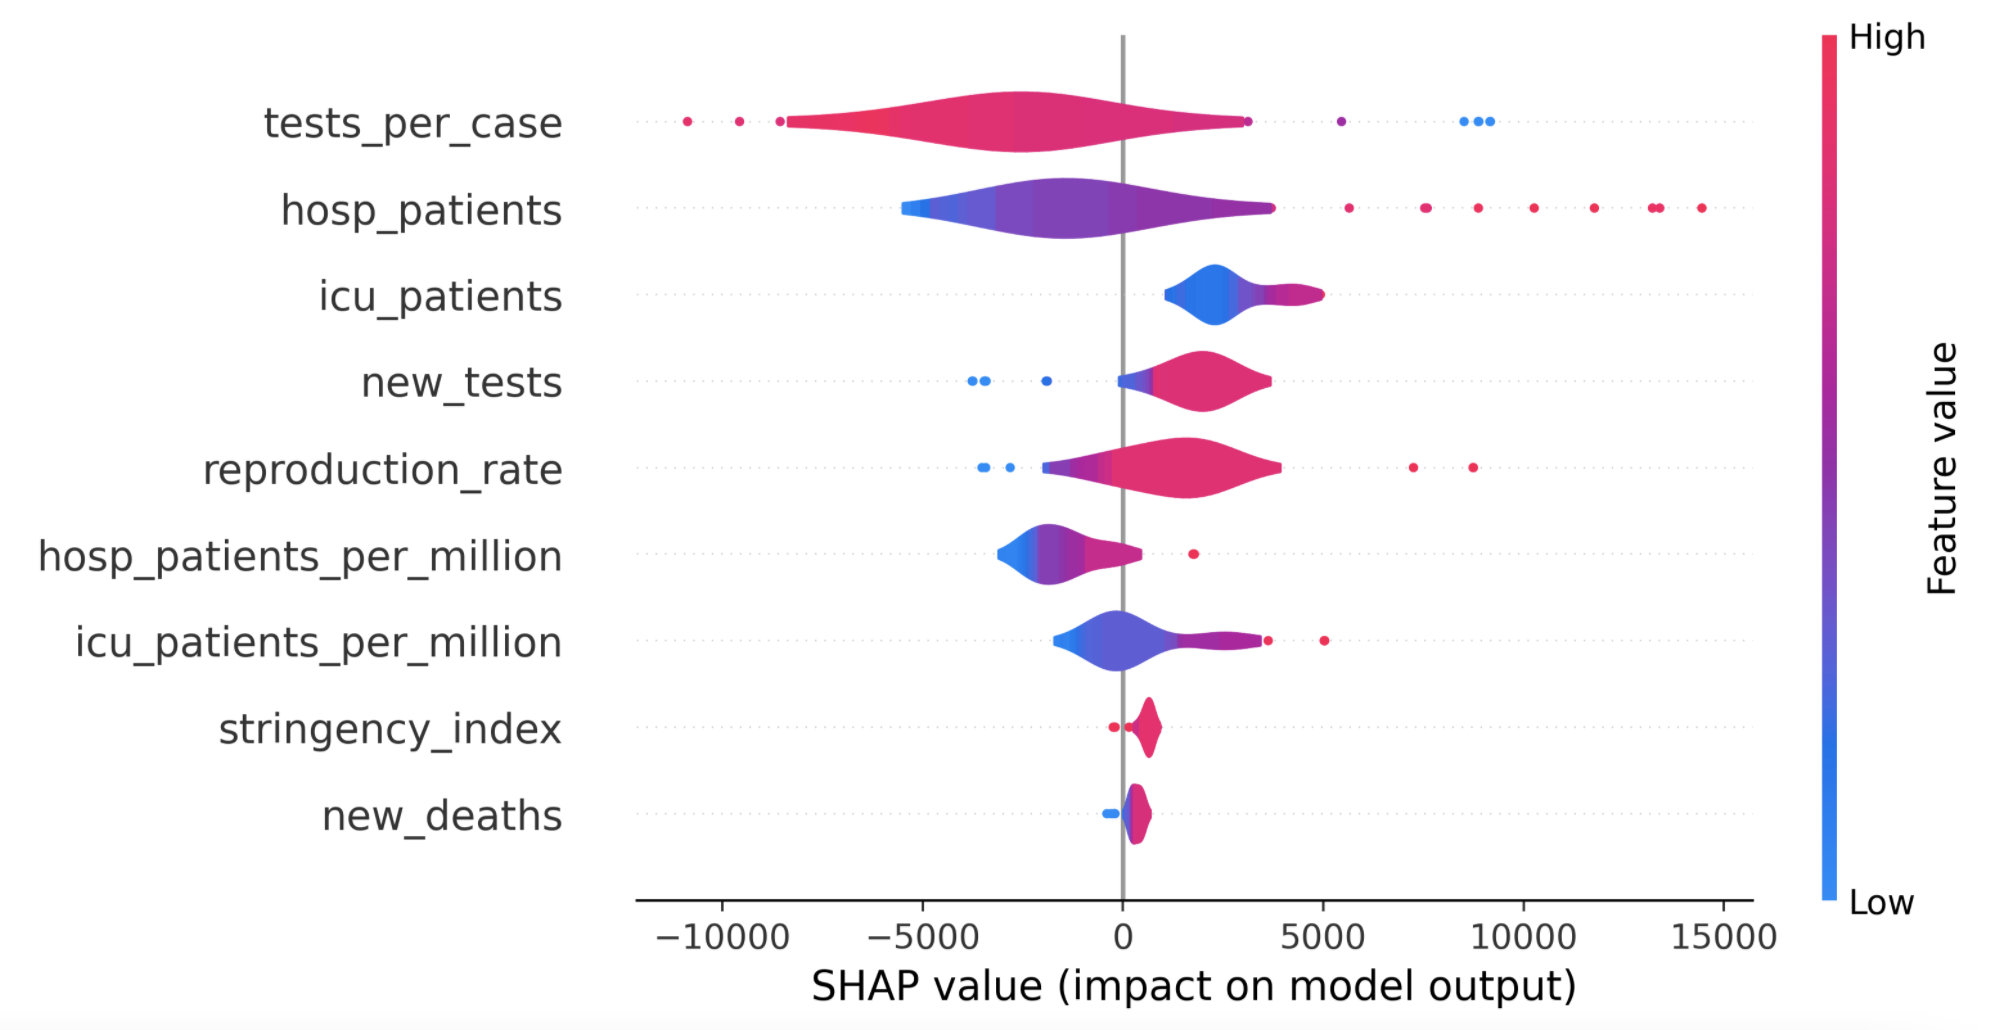
\includegraphics[width=0.6\linewidth]{../figures/shap.png} 
	\caption{Local importance - Shap values violin plot of 9 most important features.} 
\end{figure}
\subsection{ARIMA}
The selected hyperparameter for ARIMA is $p=2, d=1, q=2$, and the fitted iterative formula is:
$$\Delta Y_t = 1.1833\Delta Y_{t-1}-  0.3196\Delta Y_{t-2}-1.1550u_{t}+0.5689 u_{t-1}$$
where $\Delta Y$ represents first order difference of target variable, and $u$ is a white noise.\\

The rolling 1-step forecast for the ARIMA(2,1,2) model is as Figure 9 shows (Test RMSE = 4220.17). For long-term prediction, the precision is not expected to be good, with test RMSE equal to 11977.69, which still indicates an improvement compared to supervised models.


\begin{figure}[!htb]
	\centering
	\subfigure{
		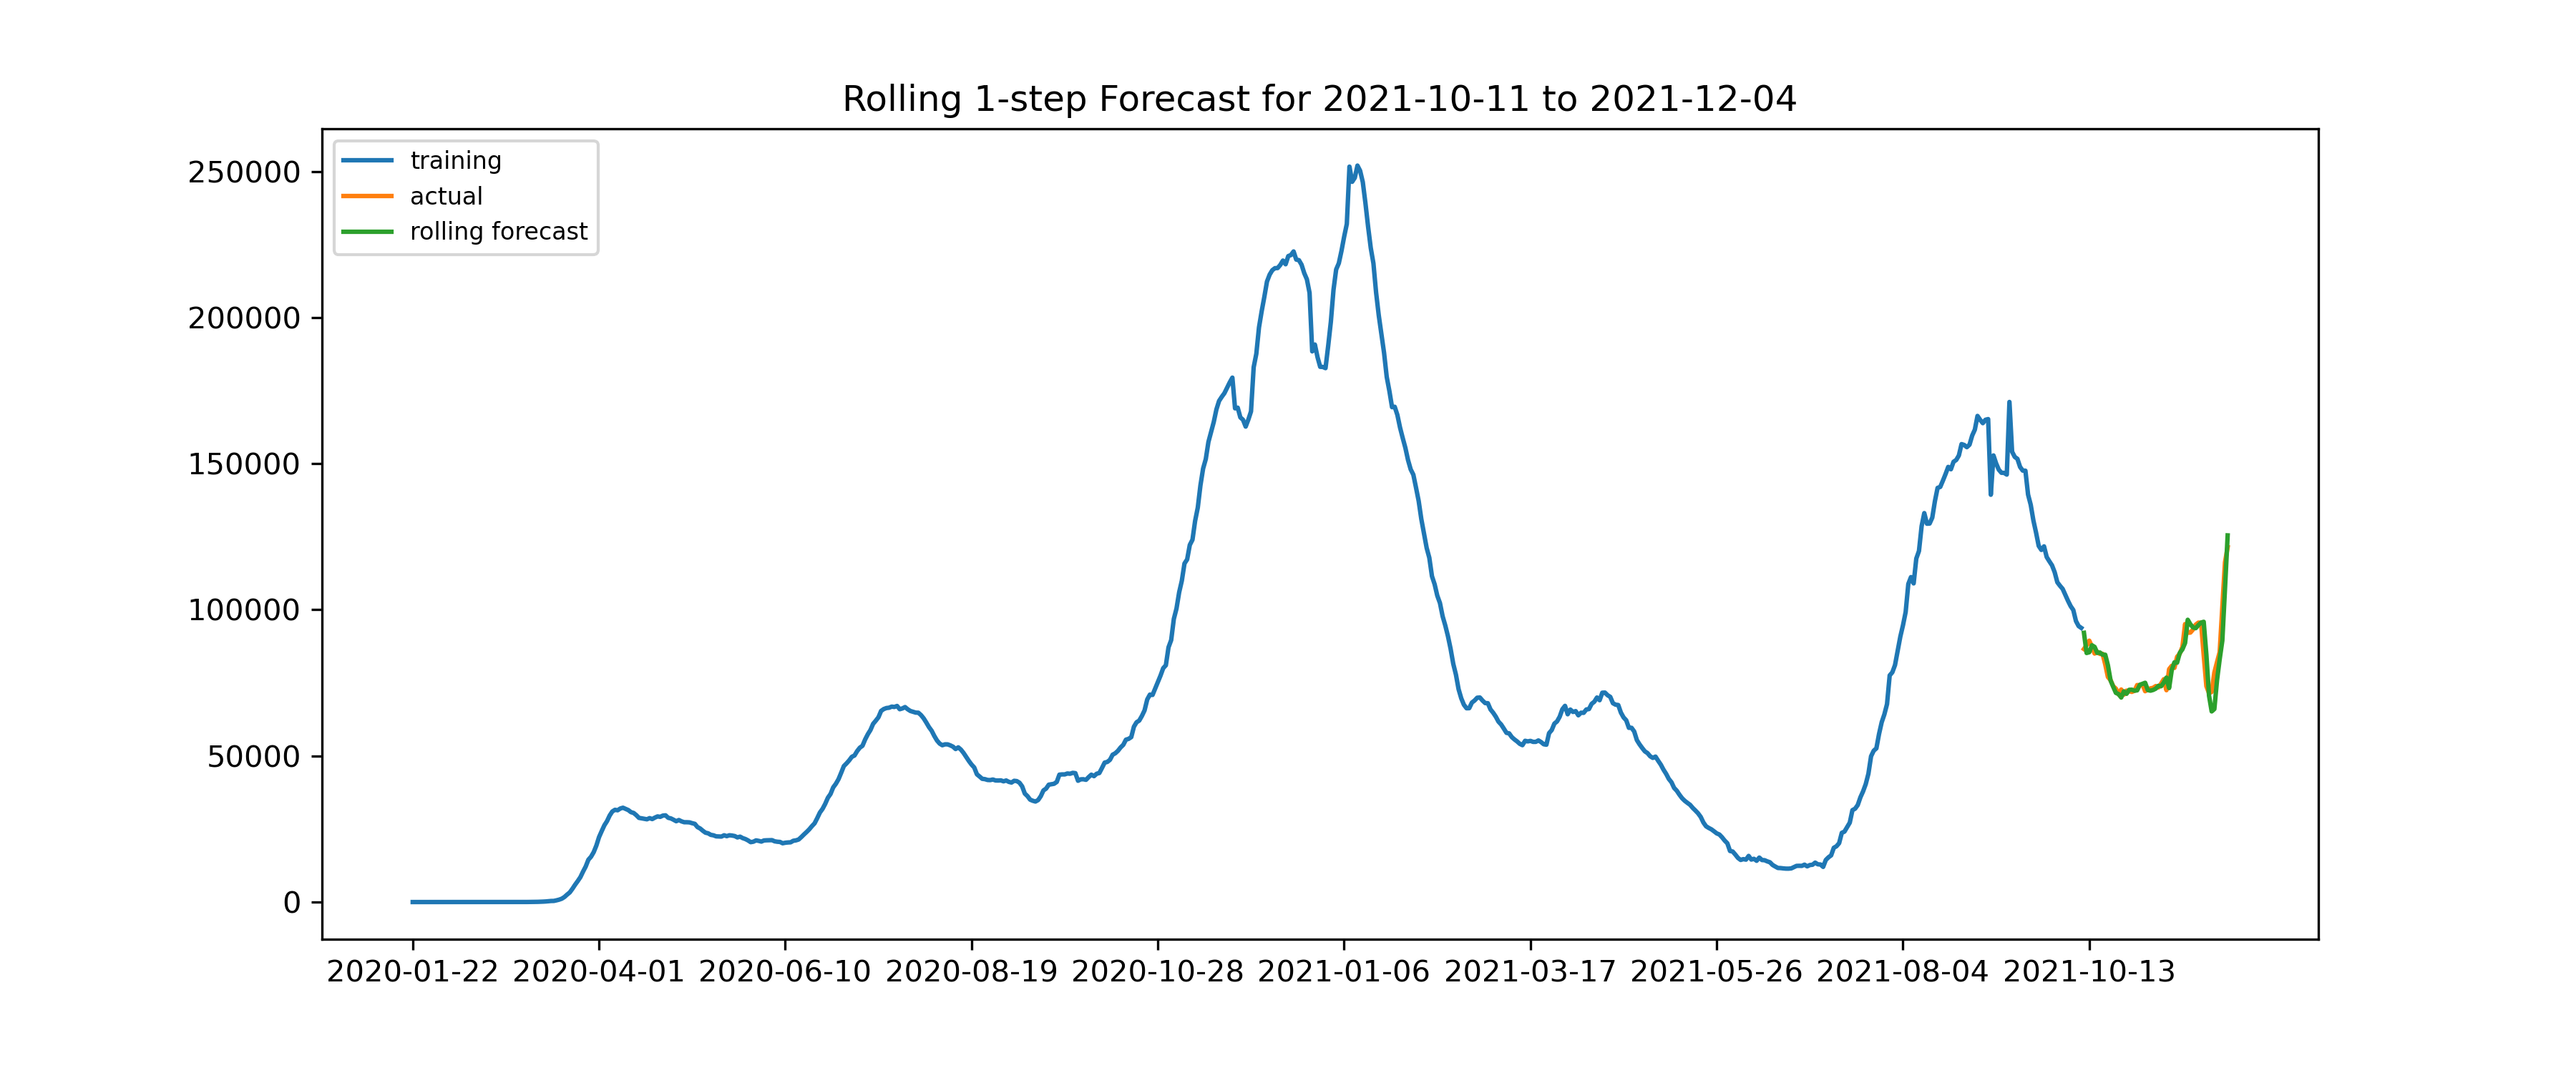
\includegraphics[width=0.9\textwidth]{../figures/ARIMA-Predict-Onestep.png}}\vspace{-0.3in}
	\subfigure{	
		\label{total cases vs. cumulated new cases} %% label for secondsubfigure
		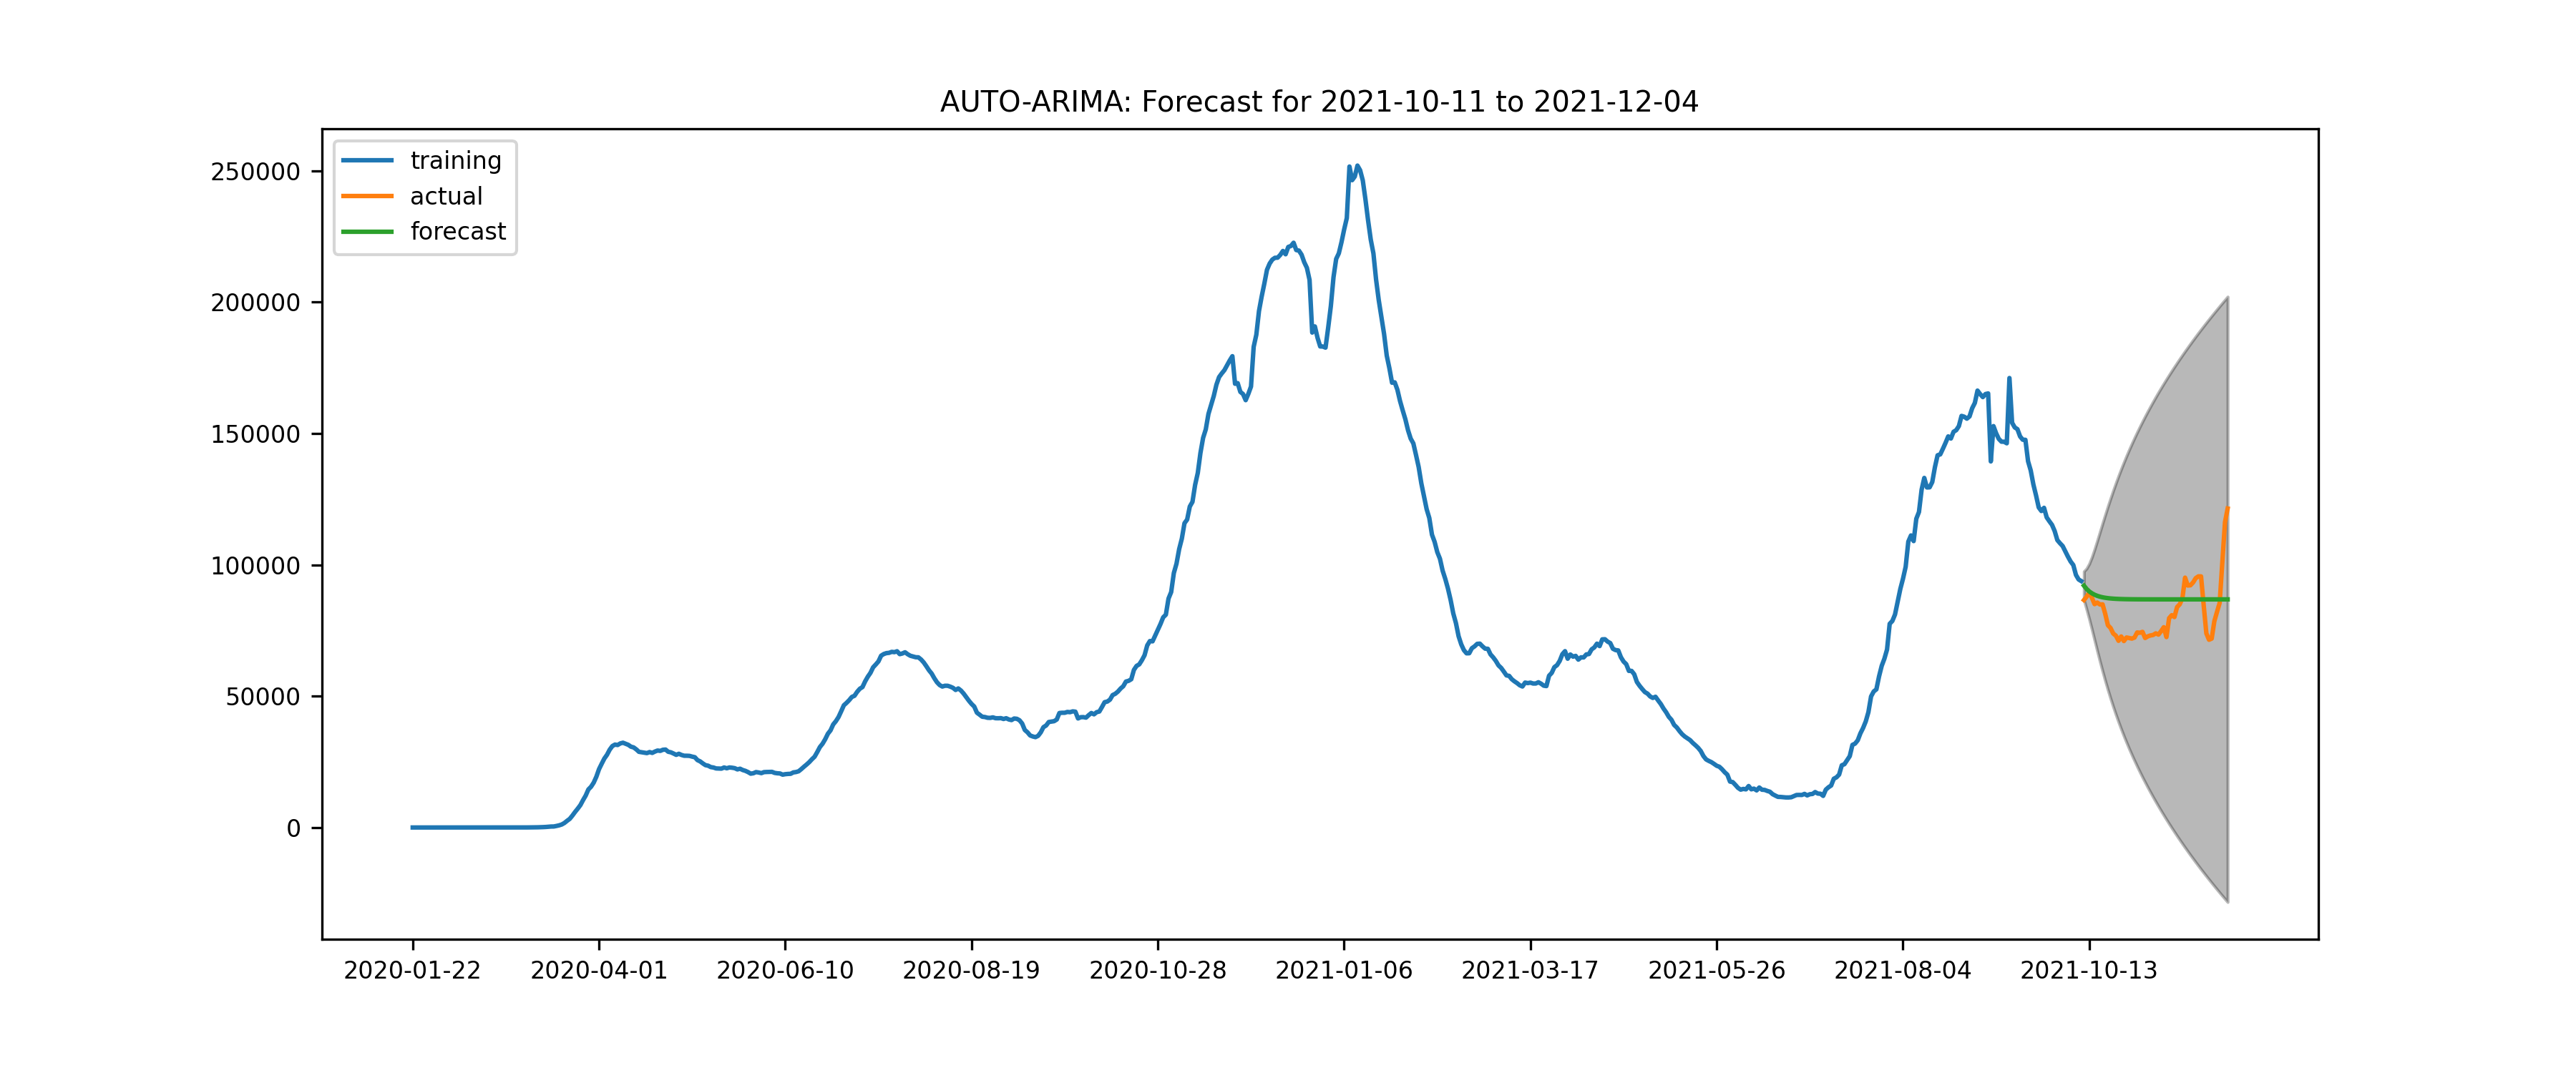
\includegraphics[width=0.9\textwidth]{../figures/ARIMA-Predict.png}}\vspace{-0.1in}
	\caption{ Long-term prediction (below) uses generated data to forecast future values. Rolling prediction (above) only moves one step, using true observations for the following data point instead of the generated points. So it won't stack the prediction error. The gray block displays the 95\% confidence area for the forecast.}
\end{figure}





\section{Outlooks}
This project compares the performance of different models on time series prediction. Supervised learning models can employ all the columns, but they assume that records are independently and identically distributed. Also, without special processing, they will ignore the group or time series structure, which is the order of data in this certain problem. These models also require access to future feature values. However, ARIMA does not require an oracle about what would the features in the future be, and it takes time structure into account. But other information in the dataset is discarded.\\

Thus, to improve the prediction model, it would be better to combine the strengths of supervised learning and time series models, developing multivariate ARIMA models. While multivariate ARIMA's ability to engage many columns as different variables is limited, fortunately, supervised learning provides a solution to select the most essential features and then only model them in multivariate ARIMA.




\newpage
\begin{thebibliography}{99}
	\bibitem{1}Ritchie, H., Mathieu, E., et al. 2020. "Coronavirus Pandemic (COVID-19)". Published online at {\em OurWorldInData.org}. Retrieved from: \url{https://ourworldindata.org/coronavirus}
	\bibitem{2}Valvo, \& Paolo S. 2020. A Bimodal Lognormal Distribution Model for the Prediction of COVID-19 Deaths" {\em Applied Sciences }10, no. 23: 8500. \url{https://doi.org/10.3390/app10238500}
	\bibitem{3} Tuli, S., Tuli, R., Gil, S S., 2020. "Predicting the growth and trend of COVID-19 pandemic using machine learning and cloud computing". {\em Internet of Things},
Volume 11,
2020,
100222,
ISSN 2542-6605,
	\url{https://doi.org/10.1016/j.iot.2020.100222}.
\end{thebibliography}

\end{document}
